% ============================================
% Chapter 5 – Implementation
% ============================================

\chapter{Implementation}

This chapter describes the practical implementation of the proposed system. 
It explains how the designed architecture was translated into working modules, 
algorithms, user interfaces, and deployment components.

% -------------------------------------------------
% 5.1 Development Environment
% -------------------------------------------------

\section{Development Environment}

This section describes the software and hardware environment used 
for system implementation.

\section{Development Environment}

This section describes the software and hardware environment used for system implementation.

\subsection{Software Environment}

\begin{itemize}
\item \textbf{IDE used:} Visual Studio Code (latest version)
\item \textbf{Programming language(s):} JavaScript, TypeScript
\item \textbf{Framework(s) used:} Next.js (latest) as a full-stack React.js framework for web, Tailwind CSS v4 for UI components, better-auth for authentication/authorization, arcjet for bot detection and rate limiting.
\item \textbf{Database system:} PostgreSQL (v18) local for local development and for production hosted on neon.com.
\item \textbf{Operating system:} Windows 11.
\item \textbf{Other tools:} Git/GitHub (latest) for version control, Microsoft PowerPoint (latest) for presentations, Microsoft Word for documents, vercel for deployment.
\end{itemize}

\subsection{Hardware Environment}

The system is developed and deployed in a web-based environment with no specific hardware dependencies beyond standard configurations.

\begin{itemize}
\item \textbf{Client-side:} Standard personal computers with input devices (keyboard, mouse) and Firefox web browsers 
\item \textbf{Hardware specifications:} 16 GB RAM, Intel Core i5 or equivalent processor, 256 GB HDD storage (no GPU required as the project is not ML-based)
\end{itemize}

% -------------------------------------------------
% 5.2 Core Module Implementation
% -------------------------------------------------

\section{Core Module Implementation}

This section explains how each major module was implemented.

\textbf{Guidelines:}
For each module:
\begin{itemize}
    \item Describe its purpose
    \item Explain key functionalities
    \item Mention important classes/functions
    \item Explain integration with other modules
\end{itemize}

\subsection{Module 1: Registration}

\textbf{Purpose:} 
To register user in the system.

\textbf{Functionality:}
Portal shows register form with inputs for name, email and password. Page shows errors as user types in inputs like valid email, name with min character length 3 and password with min 8 characters. 

\textbf{Important functions:}

\textbf{SignUp:}
When user submits form, server action parses values submitted by user, if inputs are invalid, it shows error, and function is blocked further processing to prevent malicious users calling server action. If success, then user is signed up using email, password. The session token is saved in browser for 7 days. If user uses session within 7 days, the token is refreshed automatically, and updates expiry date to next 7 days. If session token is expired, user is logged out and will need to login again.


\textbf{SendEmail:}
The system first checks if it is development environment and then logs verification link in console; otherwise if the production environment, it sends email to the user. When user clicks on the link from console or email, user is automatically logged in. The link expires in 5 minutes, if user clicks on expired link, it shows expired link and asks user to request new link for verification.

\subsection{Module 2: Login}

\textbf{Purpose:}
To login user in the system.

\textbf{Functionality:}
The system first checks if browser already has session token and is  not expired, then redirect user back to home page, because user is already logged in and no need to login again. Login form shows errors like invalid email and password length less than 8 characters as user types. It shows invalid email or password if user entered wrong credentials.

\textbf{Important functions:}

\textbf{Email verification:}
If email is already verified, then the user is automatically logged in, otherwise it shows email not verified.

\subsection{Module 3: Student Request Leave}
\textbf{Purpose:}
Allows students to formally request leave for a specific subject on a specific date. The request is reviewed by the BA and the HOD.

\textbf{Functionality:}

\begin{itemize}
\item The student selects:
\begin{itemize}
\item The subject (from currently registered courses only)
\item The lecture date.
\item Reason / description (text area)
\item Optional supporting document upload (image, max size 5 MB)
\end{itemize}
\item Real-time client-side validation is performed as the user types / selects:
\begin{itemize}
\item Duplicate check: whether the student has already submitted a leave request for the same subject on the same lecture date
\item Subject registration verification: confirms the selected subject is part of the student's current registered courses
\end{itemize}
\item If a duplicate exists, an immediate error message is displayed (e.g., You have already submitted a leave request for this lecture.'') \item On form submission, a server-side action re-validates all conditions:   \begin{itemize}   \item Subject must be offered in the current semester   \item Student must be registered in the subject   \item No existing approved / pending leave request for the same lecture   \end{itemize} \item If validation fails, the request is rejected and specific error messages are returned to the client. \item On success, a new Leave Request record is created in the database with status Pending'' and assigned to the student's Batch Advisor (BA).
\end{itemize}

\textbf{Important functions:}

\begin{itemize}
    \item Zod schema for form schema validation and in server-action for form values validation.
    \item server action validates inputs, checks permission if student is allowed to create leave request, resolves subjectId and offering and student registeration, duplicate check and then creates LR. If fails it shows error to the student.
    \item Leave request form that fetches student's enrolled subjects and renders LR form.
    \item LR form using react-hook-form with date picker with weekday + range validation; Uploader for optional image; uses useTransition + tryCatch for async UX
    \item Prisma model LeaveRequest has fields studentId, offeringId, status, date and reason.
\end{itemize}

\textbf{Integrations with other modules:}
\begin{itemize}
    \item \textbf{Subjects/Enrollment:} queries SubjectOffering enrollments to populate the subject dropdown
    \item \textbf{S3 / Uploader:} Uploader component uploads supporting images; the returned imageKey is stored on the record
    \item \textbf{Auth (Better Auth)} requireSession() ensures only authenticated users can create leave requests.
    \item \textbf{Toast:} Success/error feedback on form submission
\end{itemize}
Enrollment/subjects.

\subsection{Module 4: students announcement module:}
\textbf{Purpose:}
Displays department-targeted announcements from HODs/accountant or admin to students, with smart filtering based on the student's department, program. 

\textbf{Functionality:}
\begin{itemize}
    \item \textbf{Filtered Feed:} Shows only announcements matching the student's department / program, plus broadcasts (\verb|null| targets) 
    \item \textbf{Pin support:} Pinned announcements float to the top, newly created on the top.
    \item \textbf{Details view:} Full announcement page with image, content, author, and publish date 
    \item \textbf{Responsice Sidebar:} Right sidebar shows a preview list on student layout, which shows up in desktop screens.
    \item \textbf{Suspense + Skeletons:} Both list and detail views stream in with loading skeletons.
\end{itemize}

\textbf{Important functions:}

\begin{itemize}
\item \textbf{studentGetAllAnnouncements:} Checks resolves the student's department/program from their registration number, builds a scoped Prisma \href{vscode-file://vscode-app/d:/Programs/Microsoft\%20VS\%20Code/0870c2a0c7/resources/app/out/vs/code/electron-browser/workbench/workbench.html}{where} clause, orders by isPinned desc and createdAt desc.
    \item \textbf{studentGetAnnouncemntById:} fetches a single announcement for the detail page.
    \item Announcement details page: async RSC showing full content + optional image display.
    \item Right sidebar: wraps in Suspense on every student layout page
 
\end{itemize}
 

\textbf{Integration with other modules:}
\begin{itemize}
    \item \textbf{Auth:} requireSession identifies the student to scope announcements.
    \item \textbf{Prisma Annoucement model:} Queried with multi-dimensional AND/OR filters for targeting.
    \item \textbf{S3 /GeneralImage:} Detail page renders announcement images stored in S3 via imageKey stored in DB.
    \item Student Layout / Sidebar: Right sidebar surfaces the latest announcements passively across all student pages.
\end{itemize}

\subsection{Module 5: Student Complaints module:}
\textbf{Purpose:}
Allows students to formally raise academic or administrative complaints. Each complaint passes through a multi-stage review pipeline: BA (Batch Advisor) → HOD.

\subsubsection{Key Functionalities:}
\begin{itemize}
    \item \textbf{Create:} Title, details, category (enum), optional image upload, shows errors as user types
    \item \textbf{Update:} Editable only when status == BA PENDING
    \item \textbf{Delete:} Single or bulk delete via confirmation dialog.
    \item \textbf{Table View:} Paginated table with sort, filter by status/category/date/attachment
    \item \textbf{Details Page:} Full complaint card with HOD remarks, attachment, status badge.
\end{itemize}

\textbf{Important functions:}

\begin{itemize}
    \item zodSchema for form validation before submitting form and in server-actions to check inputs.
    \item server-action: checks Only authenticated users can submit complaint, gets department from current user data and creates complaint.
    \item Data Fetcher: fetches dynamic complaints to show on complaints page with filters, only shows student's own complaints.
\end{itemize}

\textbf{Integration with other modules:}

\begin{itemize}
    \item Permission: checks permissions to create, list, get, update:own and delete:own for complaints.
    \item Auth: only authenticated users can create complaints, gets session and resolves student by userId.
    \item S3/uploader: stores imageKey in the record.
    \item BA module: when submitted BA can view complaints submitted by their department students.
    \item nuqs: URL-synced filters in complaints page.
\end{itemize}

\subsection{Module 6: Admin user mangement:}
\textbf{Purpose:}
Admin can change any user's role, assign a department to professors, and appoint professors as Batch Advisors — each via a dedicated confirmation dialog.

\textbf{Key functionality:}
\begin{itemize}
    \item \textbf{User Listing and Filtering:} Retrieves a paginated list of platform users. It supports advanced server-side filtering by user roles, complex search queries (by name or email), and dynamic sorting, optimizing performance for large datasets.
    \item \textbf{Role Management:} Allows administrators to elevate or modify user roles (such as Professor, Accountant, Director, etc.). It automates the cleanup of old profile data and initializes new profile records atomically.
    \item \textbf{Department Assignment:} Provides the ability to assign or reassign departments to Professors, ensuring administrative structure is maintained. It includes built-in safeguards, such as preventing department reassignment for active Batch Advisors to avoid data desynchronization.
    \item \textbf{Batch Advisor Appointment:} A server-action to appoint a Professor as a Batch Advisor for their respective department. It uses business rules, such as ensuring the department does not already have an active Batch Advisor.
\end{itemize}

\textbf{Important Classes and Functions}
\begin{itemize}
    \item \textbf{getAdminUsers}: A data fetching function querying the database. It builds pagination calculations, sorting logic, and conditional search clauses.
    \item \textbf{UsersTable}: used to render users.
    \item setUserRole: A server action implementing the business logic for changing a user's role. It verifies permissions and wraps the old profile deletion and new profile creation in a single transaction.
    \item makeProfessorBatchAdvisor: server action that atomically creates a Batch Advisor record and links it to the corresponding professor and department.
\end{itemize}

\textbf{Integration with Other Modules}
\begin{itemize}
    \item \textbf{UsersTable:} Renders user data in table format with filtering and sorting using nuqs which provides URL-synced filtering.
    \item \textbf{Session Module:} All actions and data fetching use requireSession to check that user is authenticated.
    \item \textbf{requirePermission:} checks permissions to list, get and update users while changing roles checks for \texttt{user: ["set-role"]} permissions. If no permission, it redirects user to /unauthorized page.
    \item \textbf{Frontend UI Components:} The table uses dropdown for actions like view details and update user-role using confirmation dialog.
\end{itemize}

\subsection{Module 7: HOD creates ANN:}

\textbf{Purpose:}
The HOD Announcements module gives HODs to create announcements for their respective departments. Students can view the published announcements, whereas the HOD manages drafting, scheduling, ANN from their dashboard.


\textbf{Key functionality:}
\begin{itemize}
    \item \textbf{Creating Announcements}: HOD can create announcement. The creation flow includes options for tagging announcement types, pinning, and attaching images. Announcements can be published immediately or scheduled up to 2 days in the future via an automated queue using cron-jobs.
    \item \textbf{Scheduling}: Announcements can be scheduled up to two days in advance. Scheduled announcements utilize an event-driven background job (Inngest) to handle the delayed publication automatically.
    \item \textbf{Fetching Announcements}: The module implements paginated data fetching with filters. HODs can search by free text, date ranges, announcement status (e.g., Draft, Scheduled, Published), type, and attachments.
    \item \textbf{Bulk Operations}: Announcemetn Table provides convenience of bulk actions, allowing HODs to delete multiple announcements at once or update the status of several announcements simultaneously.
        \item \textbf{Displaying Details}: A dedicated drawer interface previews individual announcement details, rendering image attachments, and itemizing metadata (creation, scheduled, and published timestamps).
\end{itemize}

\textbf{Integration With Other Modules}
\begin{itemize}
    \item \textbf{Role Authentication}: verify the active user has HOD-level access to announcement operations.
    \item \textbf{Job Scheduling (Inngest)}: Integrates with the inngest client to dispatch delayed tasks managing the automated transition from Scheduled to Published states.
\end{itemize}

% -----------

% -----------

\section{Algorithm Implementation}

This section explains the implementation of the core prediction algorithm used in the system. 

\subsection{Algorithm 1: User Registration}

\textbf{Input:} User registration details including $name$, $email$, and $password$ \\
\textbf{Output:} An API response object indicating success or failure \\

The algorithm securely processes new user registrations by validating input credentials against register schema. Valid inputs are then sent to the authentication API to register a new user record.

\begin{algorithm}[H]
\caption{User Registration Process}
\begin{algorithmic}[1]

\Function{RegisterUser}{$name, email, password$}
    \State \Comment{Construct input object}
    \State $input\_data \gets \{name, email, password\}$
    
    \State \Comment{Validate input against schema}
    \State $is\_valid \gets ValidateSchema(input\_data)$
    
    \If{\textbf{not} $is\_valid$}
        \State \Return $\{status: \text{"error"}, message: \text{"Invalid form data"}\}$
    \EndIf
    
    \State \Comment{Attempt to create user via Auth API}
    \State $result \gets Call(AuthAPI.signUpEmail(name, email, password))$
    
    \If{$result.success$}
        \State \Return $\{status: \text{"success"}, message: \text{"Signup successful"}\}$
    \Else
        \State \Comment{Extract error message on failure}
        \State $error\_msg \gets ExtractErrorMessage(result.error)$
        \State \Return $\{status: \text{"error"}, message: error\_msg\}$
    \EndIf
    
\EndFunction

\end{algorithmic}
\end{algorithm}

\subsection{Algorithm 2: Reset Password}

\textbf{Input:} A user-provided $new\_password$, $confirm\_password$, and a URL $token$ \\
\textbf{Output:} An API response triggering a success toast and redirection, or an error toast \\

The algorithm captures a new password from the user alongside a secure token from their email link. It first validates that the new password meets length constraints and matches the confirmation field. Validated credentials and the token are then transmitted to the authentication client, which processes the reset and returns the specific success or error outcomes.

\begin{algorithm}[H]
\caption{Reset Password Process}
\begin{algorithmic}[1]

\State \textbf{Input:} $new\_password$, $confirm\_password$, $token$
\State \textbf{Output:} $UI\_Response$

\Function{ResetPassword}{$new\_password, confirm\_password, token$}
    \State \Comment{Construct form data}
    \State $form\_data \gets \{password: new\_password, confirmPassword: confirm\_password\}$
    
    \State \Comment{Validate against schema: matching passwords, min 8 chars}
    \State $is\_valid \gets ValidateSchema(form\_data)$
    
    \If{\textbf{not} $is\_valid$}
        \State \Return $DisplayValidationErrors()$
    \EndIf
    
    \State \Comment{Attempt password reset via Auth Client}
    \State $result \gets Call(authClient.resetPassword(new\_password, token))$
    
    \If{$result.success$}
        \State $ShowToast(\text{"Password reset successfully."})$
        \State $RedirectTo(\text{"/login"})$
        \State \Return \text{Success}
    \Else
        \State \Comment{Display specific error message from the Auth context}
        \State $ShowToast(result.error.message)$
        \State \Return \text{Failure}
    \EndIf
    
\EndFunction

\end{algorithmic}
\end{algorithm}

% -----------
% -----------

\subsection{Algorithm 3: Create Student Complaint}

\textbf{Input:} A user session, and complaint details including $title$, $details$, $category$, and optionally an $imageKey$ \\
\textbf{Output:} An API response object indicating whether the complaint creation succeeded \\

The algorithm handles the creation of a new grievance or query by a student. It enforces security by verifying the user session and ensuring the user holds the requisite permissions and is registered as a student. After confirming the user's departmental affiliation, the algorithm validates the input parameters against a strict schema before persisting the new complaint in the database linked to the student's ID and department.

\begin{algorithm}[H]
\caption{Student Complaint Creation Process}
\begin{algorithmic}[1]

\State \textbf{Input:} $input\_data$, $session$
\State \textbf{Output:} $response\_object$

\Function{CreateComplaint}{$input\_data$}
    \State \Comment{Verify active session}
    \State $session \gets RequireSession()$
    
    \State \Comment{Check specific permissions}
    \State $has\_permission \gets RequirePermission(\text{"complaints"}, \text{["create"]})$
    
    \If{\textbf{not} $has\_permission$}
        \State \Return $\{status: \text{"error"}, message: \text{"You are not allowed to create complaints"}\}$
    \EndIf
    
    \State \Comment{Fetch student record to get ID and department}
    \State $student \gets Database.Student.Find(userId: session.user.id)$
    
    \If{$student$ \textbf{is} $null$}
        \State \Return $\{status: \text{"error"}, message: \text{"Not student"}\}$
    \EndIf
    
    \State \Comment{Validate complaint input schema}
    \State $is\_valid \gets ValidateSchema(input\_data)$
    
    \If{\textbf{not} $is\_valid$}
        \State \Return $\{status: \text{"error"}, message: \text{"Invalid data"}\}$
    \EndIf
    
    \State \Comment{Persist complaint attached to the student's department}
    \State $CreationResult \gets Database.Complaint.Create($
    \State \quad $studentId: student.id,$
    \State \quad $targetDepartment: student.department,$
    \State \quad $...input\_data$
    \State $)$
    
    \If{$CreationResult.success$}
        \State \Return $\{status: \text{"success"}, message: \text{"Complaint created successfully"}\}$
    \Else
        \State \Comment{Handle exceptions safely}
        \State $error\_msg \gets ExtractErrorMessage(CreationResult.error)$
        \State \Return $\{status: \text{"error"}, message: error\_msg\}$
    \EndIf
    
\EndFunction

\end{algorithmic}
\end{algorithm}

% ---------------
% ---------------

\subsection{Algorithm 4: Submit Student Leave Request}

\textbf{Input:} A session containing the $student\_id$ and leave request data containing $date$, $reasonTitle$, $reasonDetails$, $subjectId$, and $imageKey$ \\
\textbf{Output:} An API response object indicating whether the leave request was processed and accepted \\

The algorithm captures a student's request for leave for a specific lecture session. It verifies the active user's authorization, validates the form schema and confirms the student's active enrollment in the referenced subject offering. It proactively prevents duplicate submissions.

\begin{algorithm}[H]
\caption{Submit Leave Request Process}
\begin{algorithmic}[1]

\State \textbf{Input:} $input\_data$, $student\_id$
\State \textbf{Output:} $response\_object$

\Function{SubmitLeaveRequest}{$input\_data, student\_id$}
    
    \State \Comment{Verify student has permission}
    \State $has\_permission \gets RequirePermission(\text{"leaveRequest"}, \text{["create"]})$
    
    \If{\textbf{not} $has\_permission$}
        \State \Return $\{status: \text{"error"}, message: \text{"You are not allowed to create leave requests"}\}$
    \EndIf
    
    \State \Comment{Validate input schema criteria (min lengths, valid date)}
    \State $is\_valid \gets ValidateSchema(input\_data)$
    
    \If{\textbf{not} $is\_valid$}
        \State \Return $\{status: \text{"error"}, message: \text{"Invalid data"}\}$
    \EndIf
    
    \State \Comment{Fetch the specific subject offering ID}
    \State $offering \gets Database.SubjectOffering.Find(subjectId: input\_data.subjectId)$
    
    \If{$offering$ \textbf{is} $null$}
        \State \Return $\{status: \text{"error"}, message: \text{"Subject offering not found"}\}$
    \EndIf
    
    \State \Comment{Verify the student is actually enrolled in this offering}
    \State $enrollment \gets Database.Enrollment.Find(studentId: student\_id, offeringId: offering.id)$
    
    \If{$enrollment$ \textbf{is} $null$}
        \State \Return $\{status: \text{"error"}, message: \text{"You are not enrolled in this subject"}\}$
    \EndIf
    
    \State \Comment{Prevent duplicate leave requests for the same date and offering}
    \State $existing\_request \gets Database.LeaveRequest.Find($
    \State \quad $studentId: student\_id,$
    \State \quad $offeringId: offering.id,$
    \State \quad $date: input\_data.date$
    \State $)$
    
    \If{$existing\_request$ \textbf{is not} $null$}
        \State \Return $\{status: \text{"error"}, message: \text{"A leave request for this subject and date already exists"}\}$
    \EndIf
    
    \State $CreationResult \gets Database.LeaveRequest.Create($
    \State \quad $studentId: student\_id,$
    \State \quad $date: input\_data.date,$
    \State \quad $reasonTitle: input\_data.reasonTitle,$
    \State \quad $reasonDetails: input\_data.reasonDetails,$
    \State \quad $imageKey: input\_data.imageKey,$
    \State \quad $offeringId: offering.id$
    \State $)$
    
    \If{$CreationResult.success$}
        \State \Return $\{status: \text{"success"}, message: \text{"Leave request created successfully."}\}$
    \Else
        \State \Return $\{status: \text{"error"}, message: \text{"Failed to send leave request."}\}$
    \EndIf
    
\EndFunction

\end{algorithmic}
\end{algorithm}

% ----------
% ----------

\subsection{Algorithm 5: Create HOD Announcement}

\textbf{Input:} A session and an $input\_data$ object encompassing $title$, $content$, $type$, $status$, an optional $scheduledFor$ date, an $isPinned$ flag, and an optional $imageKey$ \\
\textbf{Output:} An API response indicating either immediate or scheduled publication success, or detailed error information \\

This algorithm authenticates an HOD and validates their submission to create announcements. If scheduled the system guarantees the selected date falls between today and two days into the future.

\begin{algorithm}[H]
\caption{HOD Announcement Creation Process}
\begin{algorithmic}[1]

\State \textbf{Input:} $session$, $input\_data$
\State \textbf{Output:} $response\_object$

\Function{CreateHODAnnouncement}{$session, input\_data$}
    
    \State \Comment{Verify HOD authentication and authorization levels}
    \State $has\_permission \gets RequirePermission(\text{"announcements"}, \text{["create"]})$
    
    \If{\textbf{not} $has\_permission$}
        \State \Return $\{status: \text{"error"}, message: \text{"You are not allowed to create announcements."}\}$
    \EndIf
    
    \State \Comment{Validate structural integrity of incoming data payload}
    \State $is\_valid \gets ValidateSchema(input\_data)$
    
    \If{\textbf{not} $is\_valid$}
        \State \Return $\{status: \text{"error"}, message: \text{"Invalid form data."}\}$
    \EndIf
    
    \State \Comment{Resolve HOD profile to identify specific target department}
    \State $hod \gets Database.HOD.Find(userId: session.user.id)$
    
    \If{$hod$ \textbf{is} $null$}
        \State \Return $\{status: \text{"error"}, message: \text{"HOD profile not found."}\}$
    \EndIf
    
    \State \Comment{Validate time boundary limits for scheduling (Max 48 hours)}
    \If{$input\_data.scheduledFor$ \textbf{is not} $null$}
        \State $schedule\_date \gets input\_data.scheduledFor$
        
        \If{$schedule\_date < CurrentDate()$}
            \State \Return $\{status: \text{"error"}, message: \text{"Scheduled time must be in the future."}\}$
        \EndIf
        
        \State $max\_date \gets CurrentDate() + 2 \text{ days}$
        \If{$schedule\_date > max\_date$}
            \State \Return $\{status: \text{"error"}, message: \text{"Announcements can only be scheduled up to 2 days from now."}\}$
        \EndIf
    \EndIf
    
    \State \Comment{Create database entity referencing the resolved department}
    \State $CreationResult \gets Database.Announcement.Create($
    \State \quad $targetDepartment: hod.department,$
    \State \quad $authorId: session.user.id,$
    \State \quad $status: input\_data.scheduledFor ? \text{"SCHEDULED"} : input\_data.status,$
    \State \quad $...input\_data$
    \State $)$
    
    \If{\textbf{not} $CreationResult.success$}
        \State $error\_msg \gets ExtractErrorMessage(CreationResult.error)$
        \State \Return $\{status: \text{"error"}, message: error\_msg\}$
    \EndIf
    
    \State \Comment{Handle specialized asynchronous dispatch for delayed publication}
    \If{$input\_data.scheduledFor$ \textbf{is not} $null$}
        \State $Inngest.Send(\text{"announcement/scheduled"}, CreationResult.id, input\_data.scheduledFor)$
        \State \Return $\{status: \text{"success"}, message: \text{"Announcement scheduled for [...]"}\}$
    \EndIf
    
    \State \Return $\{status: \text{"success"}, message: \text{"Announcement created successfully."}\}$
    
\EndFunction

\end{algorithmic}
\end{algorithm}


% ----------------

\subsection{Algorithm 6: Schedule HOD Announcement}

\textbf{Input:} Inngest event payload containing the $announcementId$ and intended $scheduleDate$ \\
\textbf{Output:} An update to the specified announcement record in the database, setting its status to "PUBLISHED" at the correct time \\

This algorithm represents a durable, serverless background job managed by Inngest. It calculates the target date, strictly verifies its validity, and instructs the Inngest executor to pause the function's execution until that precise moment.

\begin{algorithm}[htbp]
\caption{HOD Scheduled Announcement Handler}
\begin{algorithmic}[1]

\State \textbf{Input:} $event\_data$ containing $announcementId$ and $scheduleDate$
\State \textbf{Output:} $confirmation\_message$

\Function{HandleAnnouncementSchedule}{$event\_data, step$}
    
    \State \Comment{Extract values from standard event payload}
    \State $announcement\_id \gets event\_data.announcementId$
    \State $target\_date \gets (event\_data.scheduleDate)$
    
    \State \Comment{Validate the parsed date to prevent runtime panics}
    \If{\textbf{not} $IsValidDate(target\_date)$}
        \State \textbf{throw} $\text{"Invalid schedule date provided for announcement."}$
    \EndIf
    
    \State \Comment{Durable execution: Pause the function state until the exactly specified time}
    \State $step.SleepUntil(target\_date)$
    
    \State \Comment{Resume execution: Isolate database mutation in a retriable step}
    \State $step.Run(\text{"publish-announcement"},$
    \State \quad \Function{Publish}{}
    \State \quad \quad $Database.Announcement.Update($
    \State \quad \quad \quad $where: \{ id: announcement\_id \},$
    \State \quad \quad \quad $data: \{$ 
    \State \quad \quad \quad \quad $status: \text{"PUBLISHED"},$ 
    \State \quad \quad \quad \quad $publishedAt: CurrentDate(),$ 
    \State \quad \quad \quad \quad $scheduledFor: null$
    \State \quad \quad \quad $\}$
    \State \quad \quad $)$
    \State \quad \EndFunction
    \State $)$
    
    \State \Return $\{ announcementId: announcement\_id, message: \text{"Announcement published!"} \}$
    
\EndFunction

\end{algorithmic}
\end{algorithm}

% -----------------

\subsection{Algorithm 7: Send System Email}

\textbf{Input:} Delivery address $to$, message $subject$, and $meta$ information containing the description and an optional link \\
\textbf{Output:} A boolean success status indicating whether the email was dispatched successfully \\

This algorithm serves as a wrapper around the Nodemailer transport service. Its primary purpose is to send email to user email, opting to log them to the console in development. In production, it formats the required text into a basic HTML template and attempts secure delivery via the configured Gmail SMTP service and sends to user email.

\begin{algorithm}[htbp]
\caption{System Email Dispatch Process}
\begin{algorithmic}[1]

\State \textbf{Input:} $to$, $subject$, $meta$
\State \textbf{Output:} $is\_successful$

\Function{SendEmail}{$to, subject, meta$}
    
    \State \Comment{Development Guard: Intercept emails to prevent external spam}
    \If{$Environment.NODE\_ENV \neq \text{"production"}$}
        \State $Console.Log(\text{"[DEV EMAIL]"}, \{to, subject, meta\})$
        \State \Return $\{ success: \textbf{true} \}$
    \EndIf
    
    \State \Comment{Construct secure HTML email body using pre-defined styles}
    \State $html\_body \gets \text{GenerateHTMLTemplate}(subject, meta.description, meta.link)$
    
    \State $mail\_options \gets \{$
    \State \quad $from: Environment.NODEMAILER\_USER,$
    \State \quad $to: to,$
    \State \quad $subject: subject,$
    \State \quad $html: html\_body$
    \State $\}$
    
    \State \Comment{Attempt transmission via Nodemailer Transport (Gmail SMTP)}
    \State $TransmissionResult \gets Call(transporter.sendMail(mail\_options))$
    
    \If{$TransmissionResult.success$}
        \State \Return $\{ success: \textbf{true} \}$
    \Else
        \State \Comment{Swallow raw transport errors to prevent internal leakage}
        \State \Return $\{ success: \textbf{false} \}$
    \EndIf
    
\EndFunction

\end{algorithmic}
\end{algorithm}

% ---------------

\subsection{Algorithm 8: Batch Advisor Complaint Review}

\textbf{Input:} complaints submitted by students of BA which are pending \\
\textbf{Output:} An update to the specified complaint record transitioning its status and saving the advisor's remarks \\

This algorithm maps the initial stage of a student's complaints flow. When a new submission arrives, its status defaults to \textit{BA\_PENDING} and is routed to the corresponding department. The BA retrieves these pending items and adds remarks. If rejected, the COMPL is halted permanently. If accepted, the status escalates to \textit{HOD\_PENDING}, awaiting final decision from the Head of Department. Both outcomes log the advisor's remarks and a precise review timestamp.

\begin{algorithm}[htbp]
\caption{Batch Advisor Decision Workflow}
\begin{algorithmic}[1]

\State \textbf{Input:} $session$, $complaint\_id$, $is\_accepted$, $remarks$
\State \textbf{Output:} $updated\_complaint$

\Function{ReviewComplaintAsBatchAdvisor}{$session, complaint\_id, is\_accepted, remarks$}
    
    \State \Comment{Authorize Batch Advisor access}
    \State $has\_permission \gets RequirePermission(\text{"complaints"}, \text{["update"]})$
    
    \If{\textbf{not} $has\_permission$}
        \State \Return $\{status: \text{"error"}, message: \text{"Unauthorized access"}\}$
    \EndIf
    
    \State \Comment{Identify the advisor's specific department scope}
    \State $advisor \gets Database.BatchAdvisor.Find(userId: session.user.id)$
    
    \If{$advisor$ \textbf{is} $null$}
        \State \Return $\{status: \text{"error"}, message: \text{"Advisor profile not found."}\}$
    \EndIf
    
    \State \Comment{Query the specific complaint within the advisor's department queue}
    \State $complaint \gets Database.Complaint.Find($
    \State \quad $id: complaint\_id,$
    \State \quad $targetDepartment: advisor.department,$
    \State \quad $status: \text{"BA\_PENDING"}$
    \State $)$
    
    \If{$complaint$ \textbf{is} $null$}
        \State \Return $\{status: \text{"error"}, message: \text{"Complaint not found or already processed."}\}$
    \EndIf
    
    \State \Comment{Determine escalation or termination based on advisor action}
    \If{$is\_accepted$}
        \State $new\_status \gets \text{"HOD\_PENDING"}$
    \Else
        \State $new\_status \gets \text{"BA\_REJECTED"}$
    \EndIf
    
    \State \Comment{Log the decision and escalate}
    \State $UpdateResult \gets Database.Complaint.Update($
    \State \quad $where: \{ id: complaint.id \},$
    \State \quad $data: \{$
    \State \quad \quad $status: new\_status,$
    \State \quad \quad $baRemarks: remarks,$
    \State \quad \quad $baReviewedAt: CurrentDate()$
    \State \quad $\}$
    \State $)$
    
    \If{$UpdateResult.success$}
        \State \Return $\{status: \text{"success"}, message: \text{"Action recorded successfully."}\}$
    \Else
        \State \Return $\{status: \text{"error"}, message: \text{"Database update failed."}\}$
    \EndIf
    
\EndFunction

\end{algorithmic}
\end{algorithm}

% --------------

\subsection{Algorithm 9: Head of Department Complaint Review}

\textbf{Input:} A user session belonging to an HOD, the $complaint\_id$, and a review decision ($is\_accepted$, $is\_reassigned$, along with optional $remarks$ and a $newDepartment$) \\
\textbf{Output:} An update to the specified complaint record culminating in final acceptance, rejection, or reassignment \\

This algorithm maps the conclusive stage of a student's complaint's status. When a BA forwards a verified complaint, its status transitions to \textit{HOD\_PENDING}. The HOD assesses the COMPL. Rejection permanently halts the COMPL. Acceptance marks the complaint as successfully resolved (\textit{HOD\_ACCEPTED}). Crucially, if the complaint was incorrectly routed, the HOD can reassign the ticket to a new target department, resetting its state back to \textit{BA\_PENDING} within that new department's queue.

\begin{algorithm}[H]
\caption{HOD Decision Workflow}
\begin{algorithmic}[1]

\State \textbf{Input:} $complaint\_id$, $is\_accepted$, $is\_reassigned$, $new\_dept$
\State \textbf{Output:} $updated\_complaint$

\Function{ReviewComplaintAsHOD}{$id, is\_accepted, is\_reassigned$}
    
    \State \Comment{Query specific escalated complaint}
    \State $complaint \gets Database.Complaint.Find(id, \text{"HOD\_PENDING"})$
    
    \If{$is\_reassigned$}
        \State \Comment{Handle Reassignments}
        \State $Database.Complaint.Update(id, \{status: \text{"BA\_PENDING"}, dept: new\_dept\})$
        \State \Return $\text{"Complaint reassigned."}$
    \EndIf
    
    \State \Comment{Determine escalation or termination}
    \If{$is\_accepted$}
        \State $new\_status \gets \text{"HOD\_ACCEPTED"}$
    \Else
        \State $new\_status \gets \text{"HOD\_REJECTED"}$
    \EndIf
    
    \State \Comment{Log the final decision}
    \State $Database.Complaint.Update(id, \{status: new\_status\})$
    \State \Return $\text{"Final action recorded."}$
    
\EndFunction

\end{algorithmic}
\end{algorithm}

% --------------
% --------------

\subsection{Algorithm 10: Appoint Batch Advisor}

\textbf{Input:} A user session belonging to an Admin, the target user's $userId$, and their specified $department$ \\
\textbf{Output:} An update to the specified user's roles and database profiles, elevating them to Batch Advisor for that department \\

This algorithm maps the admin process of appointing a new BA. Because Batch Advisors are inherently tied to specific departments, they must first exist as Professors within those departments. It checks assigning an advisor to a department that already has one.

\begin{algorithm}[H]
\caption{Batch Advisor Appointment Workflow}
\begin{algorithmic}[1]

\State \textbf{Input:} $userId$, $department$
\State \textbf{Output:} $success\_status$

\Function{AppointBatchAdvisor}{$userId, department$}
    
    \State \Comment{Step 1: Verify Administrative Access}
    \State $has\_permission \gets RequirePermission(\text{"user"}, \text{["set-role"]})$
    
    \If{\textbf{not} $has\_permission$}
        \State \Return $\{status: \text{"error"}, message: \text{"Unauthorized access"}\}$
    \EndIf
    
    \State \Comment{Step 2: Ensure User is a Professor}
    \State $user \gets Database.User.Find(userId)$
    \If{$user.role \neq \text{"PROFESSOR"}$}
        \State \Comment{Delete conflicting profiles and create Professor profile record}
        \State $Database.ExecuteTransaction($
        \State \quad $UpdateUserRole(userId, \text{"PROFESSOR"}),$
        \State \quad $CreateProfessorProfile(userId, GenerateEmployeeNo()),$
        \State \quad $DeleteOtherProfiles(userId)$
        \State $)$
    \EndIf
    
    \State \Comment{Step 3: Assign Department to Professor Profile}
    \State $professor \gets Database.Professor.Find(userId)$
    \If{$professor.department \neq department$}
        \State $Database.Professor.Update(userId, \{ department: department \})$
    \EndIf
    
    \State \Comment{Step 4: Execute Batch Advisor Appointment Checks}
    \If{$professor.batchAdvisor$ \textbf{is not} $null$}
        \State \Return $\{status: \text{"error"}, message: \text{"User is already a Batch Advisor."}\}$
    \EndIf
    
    \State $existing\_ba \gets Database.BatchAdvisor.Find(\{ department \})$
    \If{$existing\_ba$ \textbf{is not} $null$}
        \State \Return $\{status: \text{"error"}, message: \text{"Department already has a Batch Advisor."}\}$
    \EndIf
    
    \State \Comment{Step 5: Atomic Transaction to Link Profiles}
    \State $Database.ExecuteTransaction($
    \State \quad $Database.BatchAdvisor.Create($
    \State \quad \quad $userId: userId,$
    \State \quad \quad $professorId: professor.id,$
    \State \quad \quad $department: department$
    \State \quad $),$
    \State \quad $Database.Professor.Update(userId, \{ batchAdvisorId: userId \})$
    \State $)$
    
    \State \Return $\{status: \text{"success"}, message: \text{"Appointed as Batch Advisor."}\}$
    
\EndFunction

\end{algorithmic}
\end{algorithm}

% --------------
% --------------

\subsection{Algorithm 11: Create Offering and Assign Professor}

\textbf{Input:} Target subject configuration parameters ($subjectId, semester, year, totalLectures, department$) alongside a selected $professorId$  \\
\textbf{Output:} The generated $offeringId$ and a success status if the professor is successfully bound to the new offering \\

This algorithm breaks down the two-step process conducted by an Administrator to launch a new academic offering. First, it validates that the proposed offering (e.g., specific semester and year for a specific subject in a department) does not already exist to prevent database duplication. Upon successfully creating the base offering, the second stage triggers: binding a faculty member to that specific classroom via an atomic upsert operation on the TeachingAssignment table.

\begin{algorithm}[H]
\caption{Offering Creation Workflow (Part 1: Validation and Initialization)}
\begin{algorithmic}[1]

\State \textbf{Input:} $offering\_params$, $professor\_id$
\State \textbf{Output:} $offering\_id, assignment\_status$

\Function{CreateAndAssignOffering}{$offering\_params, professor\_id$}
    
    \State \Comment{Step 1: Verify Administrative Access for Creation}
    \State $can\_create \gets RequirePermission(\text{"subjectOfferings"}, \text{["create"]})$
    
    \If{\textbf{not} $can\_create$}
        \State \Return $\{status: \text{"error"}, message: \text{"Unauthorized access"}\}$
    \EndIf
    
    \State \Comment{Validate against duplication}
    \State $existing\_count \gets Database.SubjectOffering.Count($
    \State \quad $year: offering\_params.year,$
    \State \quad $semester: offering\_params.semester,$
    \State \quad $subjectId: offering\_params.subjectId,$
    \State \quad $department: offering\_params.department$
    \State $)$
    
    \If{$existing\_count > 0$}
        \State \Return $\{status: \text{"error"}, message: \text{"This offering already exists."}\}$
    \EndIf
    
    \State \Comment{Step 2: Initialize Base Offering}
    \State $new\_offering \gets Database.SubjectOffering.Create(offering\_params)$
    
    \State \Comment{Step 3: Proceed to Faculty Assignment}
    \State $AssignmentResult \gets Call($ \Call{AssignTeacherToOffering}{$new\_offering.id, professor\_id$} $)$
    
    \If{$AssignmentResult.success$}
        \State \Return $\{status: \text{"success"}, offeringId: new\_offering.id\}$
    \Else
        \State \Return $\{status: \text{"partial\_error"}, message: AssignmentResult.message\}$
    \EndIf
    
\EndFunction

\end{algorithmic}
\end{algorithm}

\begin{algorithm}[H]
\caption{Offering Creation Workflow (Part 2: Faculty Assignment)}
\begin{algorithmic}[1]

\Function{AssignTeacherToOffering}{$offering\_id, professor\_id$}
    
    \State \Comment{Verify Administrative Access for Assignment}
    \State $can\_assign \gets RequirePermission(\text{"subjectOfferings"}, \text{["update"]})$
    
    \If{\textbf{not} $can\_assign$}
        \State \Return $\{status: \text{"error"}, message: \text{"Unauthorized access"}\}$
    \EndIf
    
    \State \Comment{Bind professor to offering cleanly using an Upsert}
    \State $Database.TeachingAssignment.Upsert($
    \State \quad $where: \{ offeringId: offering\_id \},$
    \State \quad $update: \{ professorId: professor\_id \},$
    \State \quad $create: \{ offeringId: offering\_id, professorId: professor\_id \}$
    \State $)$
    
    \State \Return $\{status: \text{"success"}, message: \text{"Teacher assigned successfully."}\}$
\EndFunction

\end{algorithmic}
\end{algorithm}

% ------------
% ------------



% ------------
% ------------
% ------------

\section{External APIs / SDKs}
\begin{table}[H]
    \centering
    \renewcommand{\arraystretch}{1.5}
    \begin{tabular}{|p{3cm}|p{8cm}|p{4cm}|}
        \hline
        \textbf{API/SDK Name} & \textbf{Purpose} & \textbf{Used In Module} \\
        \hline
        \textbf{Inngest} & 
        Provides serverless background jobs and scheduled task execution. It is utilized to handle asynchronous event-driven workflows, such as pausing execution to publish announcements at a scheduled date after a specific time limit. \newline
        \textbf{Authentication:} Authenticates with the Inngest platform via environment-level API keys (implicit in the SDK setup). & 
        Scheduling Module \\
        \hline
    \end{tabular}
    \caption{External APIs and SDKs Used (Part 1)}
    \label{tab:external_apis_1}
\end{table}

\begin{table}[H]
    \centering
    \renewcommand{\arraystretch}{1.5}
    \begin{tabular}{|p{3cm}|p{8cm}|p{4cm}|}
        \hline
        \textbf{API/SDK Name} & \textbf{Purpose} & \textbf{Used In Module} \\
        \hline
        \textbf{Better-Auth} & 
        Acts as the primary comprehensive authentication and authorization framework. It manages the full user lifecycle including sign-up, email/password login, email verification, password resets, and secure session management. It also integrates Role-Based Access Control (RBAC) to enforce permissions across different user roles (e.g., Admin, Student, Professor). \newline
        \textbf{Authentication:} Utilizes secure HTTP-only Next.js cookies and database-backed sessions via a Prisma PostgreSQL adapter. & 
        User Management / Authentication Module \\
        \hline
        \textbf{Nodemailer} & 
        Handles the reliable delivery of outgoing transactional emails. It is invoked programmatically to send critical communications to users, such as email verification links upon registration, password reset links, and role assignment notifications. \newline
        \textbf{Authentication:} Authenticates with an external SMTP server using standard credentials (email and application password) injected via environment variables. & 
        Email verifications/ register \\
        \hline
    \end{tabular}
    \caption{External APIs and SDKs Used (Part 2)}
    \label{tab:external_apis_2}
\end{table}


% -------------------------------------------------
% 5.5 User Interface Implementation
% ------------------------------------------------

\section{User Interface Implementation}

This section presents a detailed explanation of all user interface screens 
developed for the system. Each screen is discussed in terms of its purpose, 
functionalities, navigation flow, validations, and integration with backend modules.

Students are required to include screenshots of every major screen 
implemented in the system.

% -------------------------------------------------
% 5.5.1 UI Design Approach
% -------------------------------------------------

\subsection{UI Design Approach}

The project utilizes shadcn/ui, a collection of beautifully designed, copy-pasteable components built on Radix UI primitives and Tailwind CSS. The design follows a modern minimalist philosophy emphasizing ``less is more'' with clean, uncluttered interfaces, ample white space, subtle shadows for depth and hierarchy. This creates sleek, elegant UIs that distinct from heavier systems like Material Design.

\textbf{UI/UX methodology} centers on developer-owned, composable components with beautiful defaults that ensure unified appearance out-of-the-box. Components are designed to naturally fit together as a consistent system, promoting rapid iteration, customization via design tokens (CSS variables for colors, spacing, radii), and a utility-first Tailwind workflow.

Wireframes were create using Google stitch, and further design decisions were made while implementing.

\textbf{Consistency in color scheme and typography} is maintained through a centralized theming system using CSS variables and Tailwind configuration. A simple, restrained palette (often neutral base with accent colors) ensures visual harmony, while typography relies on limited sizes (typically 4 levels) and weights (semibold for emphasis, regular for body) via utility classes, avoiding shipped styles to allow full project control.

\textbf{Accessibility considerations} draw from Radix UI's foundation, using built-in keyboard navigation, focus management, ARIA attributes, screen reader support, high-contrast ratios (where customized), and reduced-motion preferences. Components aim for WCAG compliance, though final accessibility depends on implementation choices like proper semantic usage and alt text.

\textbf{Responsive design strategy} adopts a mobile-first approach leveraging Tailwind's responsive utilities (breakpoints: sm 640px, md 768px, lg 1024px, xl 1280px, etc.). Components adapt fluidly via classes like sm md, ensuring seamless scaling across devices with adaptive patterns (e.g., collapsible navigation, drawers on mobile).

Overall, the approach delivers a clean, accessible, themeable, and performant interface aligned with current minimalist web trends.


% -------------------------------------------------
% 5.5.2 Screen-wise Implementation
% -------------------------------------------------

\subsection{Screen-wise Implementation}

Each major screen explains following structure:

\begin{itemize}
    \item \textbf{Purpose of Screen}
    \item \textbf{Main Components (Buttons, Forms, Lists, Cards)}
    \item \textbf{User Interaction Flow}
    \item \textbf{Backend/API Integration}
    \item \textbf{Validation and Error Handling}
\end{itemize}

% ==============

\subsubsection{Screen 1: Register Screen}

\textbf{Purpose:}
This screen enables new unauthenticated users to create an account in the system by providing their essential details.

\textbf{Components:} 
\begin{itemize} 
    \item Name field
    \item Email field
    \item Password field
    \item Register button
    \item Login link (for existing users) 
\end{itemize}

\textbf{Functional Flow:} The user enters their name, email, and password. Upon clicking the Register button, a loading spinner is displayed to indicate the submission is in progress. If the registration is successful, a confirmation toast notification appears and the user is redirected to a success page /register/success. If it fails, an error toast notification is displayed.

\textbf{Backend Integration:} The form submission triggers a signUp server action. This action processes the credentials securely on the backend. The request is managed using a useTransition hook for state updates to handle asynchronous execution without blocking the client.

\textbf{Validation:} Client-side validation is enforced in real-time using react-hook-form integrated with a Zod schema. Each field checks for input validity on change, displaying specific inline error messages and applying ARIA invalid attributes if the requirements (e.g., proper email format, minimum password length) are not met.

\begin{center}
  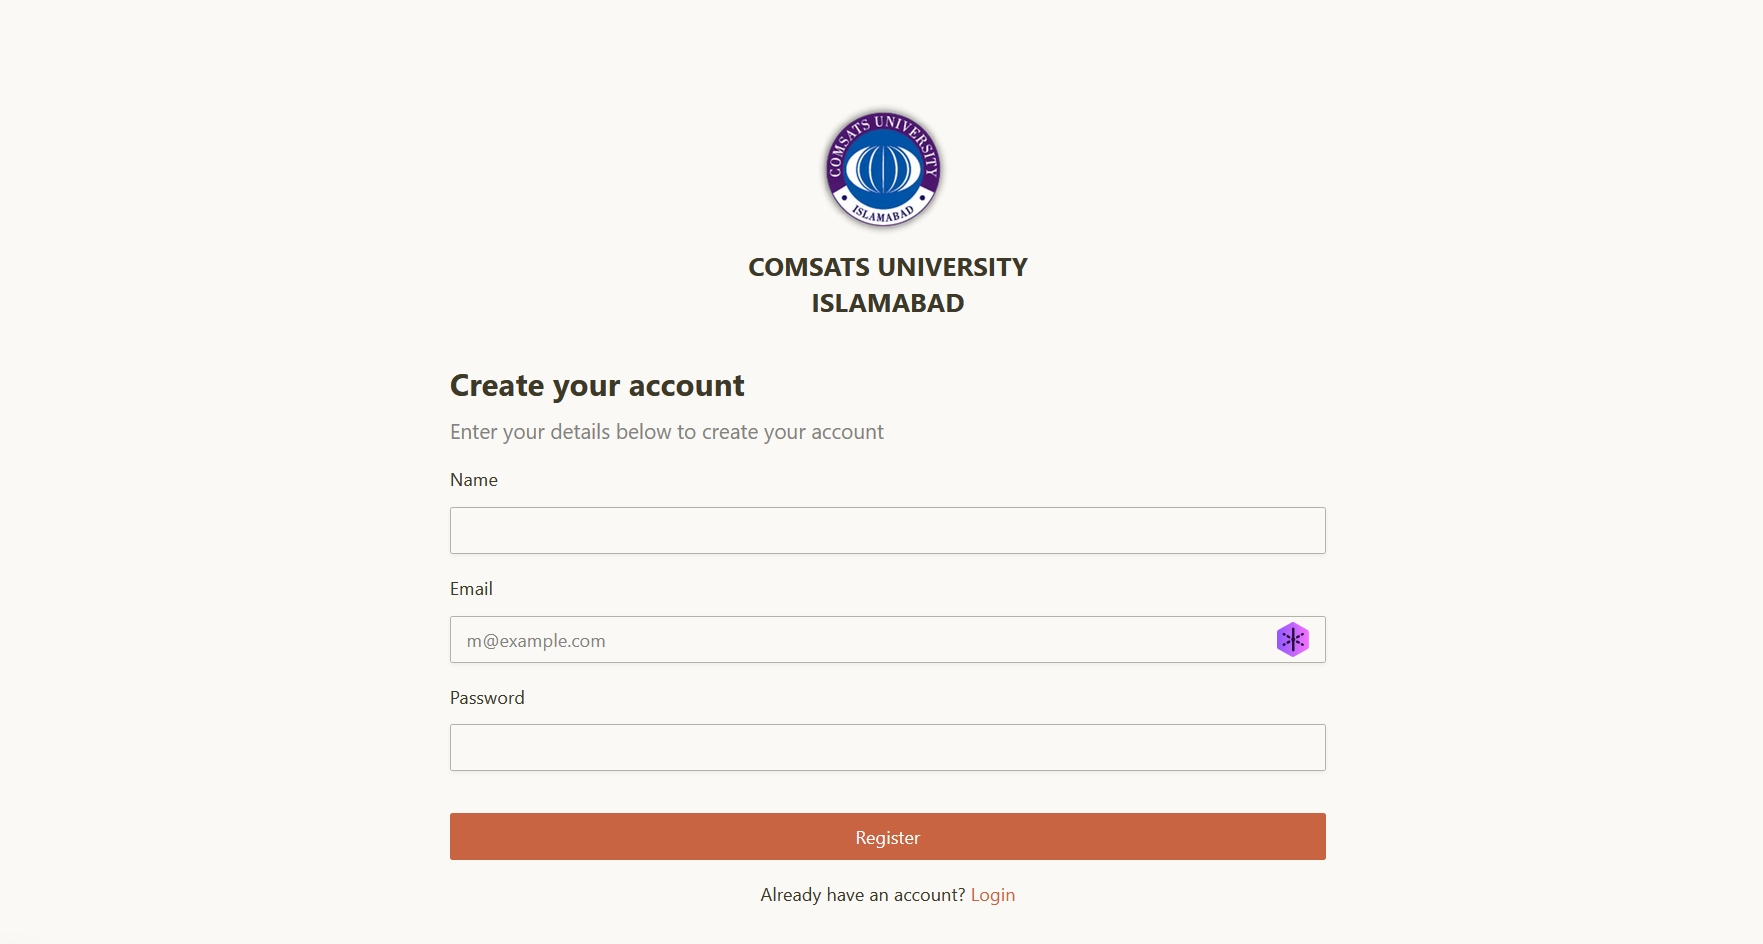
\includegraphics[width=\linewidth]{Figures/web/reg.png}
  \smallskip
  \textbf{Figure X:} Register Screen.
\end{center}


% -------------------------------------------------

\subsubsection{Screen 2: Student Dashboard Screen}

\textbf{Purpose:}
This screen serves as the primary landing page for authenticated students. It provides an immediate academic overview, displaying all the subjects the student is currently enrolled in, along with their high-level details and attendance status.

\textbf{Components:} 
\begin{itemize}
    \item Welcome greeting
    \item Responsive grid layout for subject cards \item 
    \textbf{Subject Card:}    
    \begin{itemize} 
        \item Subject Name and Credit Hours badge
        \item Subject Code, Teacher Name, and Class Name
        \item Attendance section (Link to detailed attendance, percentage, and visual progress bar)
        \item Conditional warning message for low attendance
    \end{itemize}
\end{itemize}

\textbf{Functional Flow:} Upon logging in, the student is redirected to the dashboard. The page automatically fetches the student's enrolled subjects. The subjects are displayed as cards in a responsive grid. The user can view their current attendance percentage for each subject. If attendance falls below the \text{80} threshold, the progress bar turns red and a warning message ("⚠️ Below minimum requirement") is displayed. The user can click the "Attendance" link on any card to navigate to the detailed attendance page for that specific subject.

\textbf{Backend Integration:} The screen uses React Server Components (RSC) to asynchronously fetch the student's subjects using the getStudentSubjects data access function before rendering the page. This ensures the data is loaded securely on the server without exposing API endpoints directly to the client.

\textbf{Validation:} The SubjectCard component includes conditional rendering logic to validate the \texttt{attendancePercentage}. If the value is strictly less than 80, it applies critical (red) styling to the text and progress bar, and displays a specific warning message to alert the student. Otherwise, it uses success (green) styling for the attendance indicators.

\begin{center}
  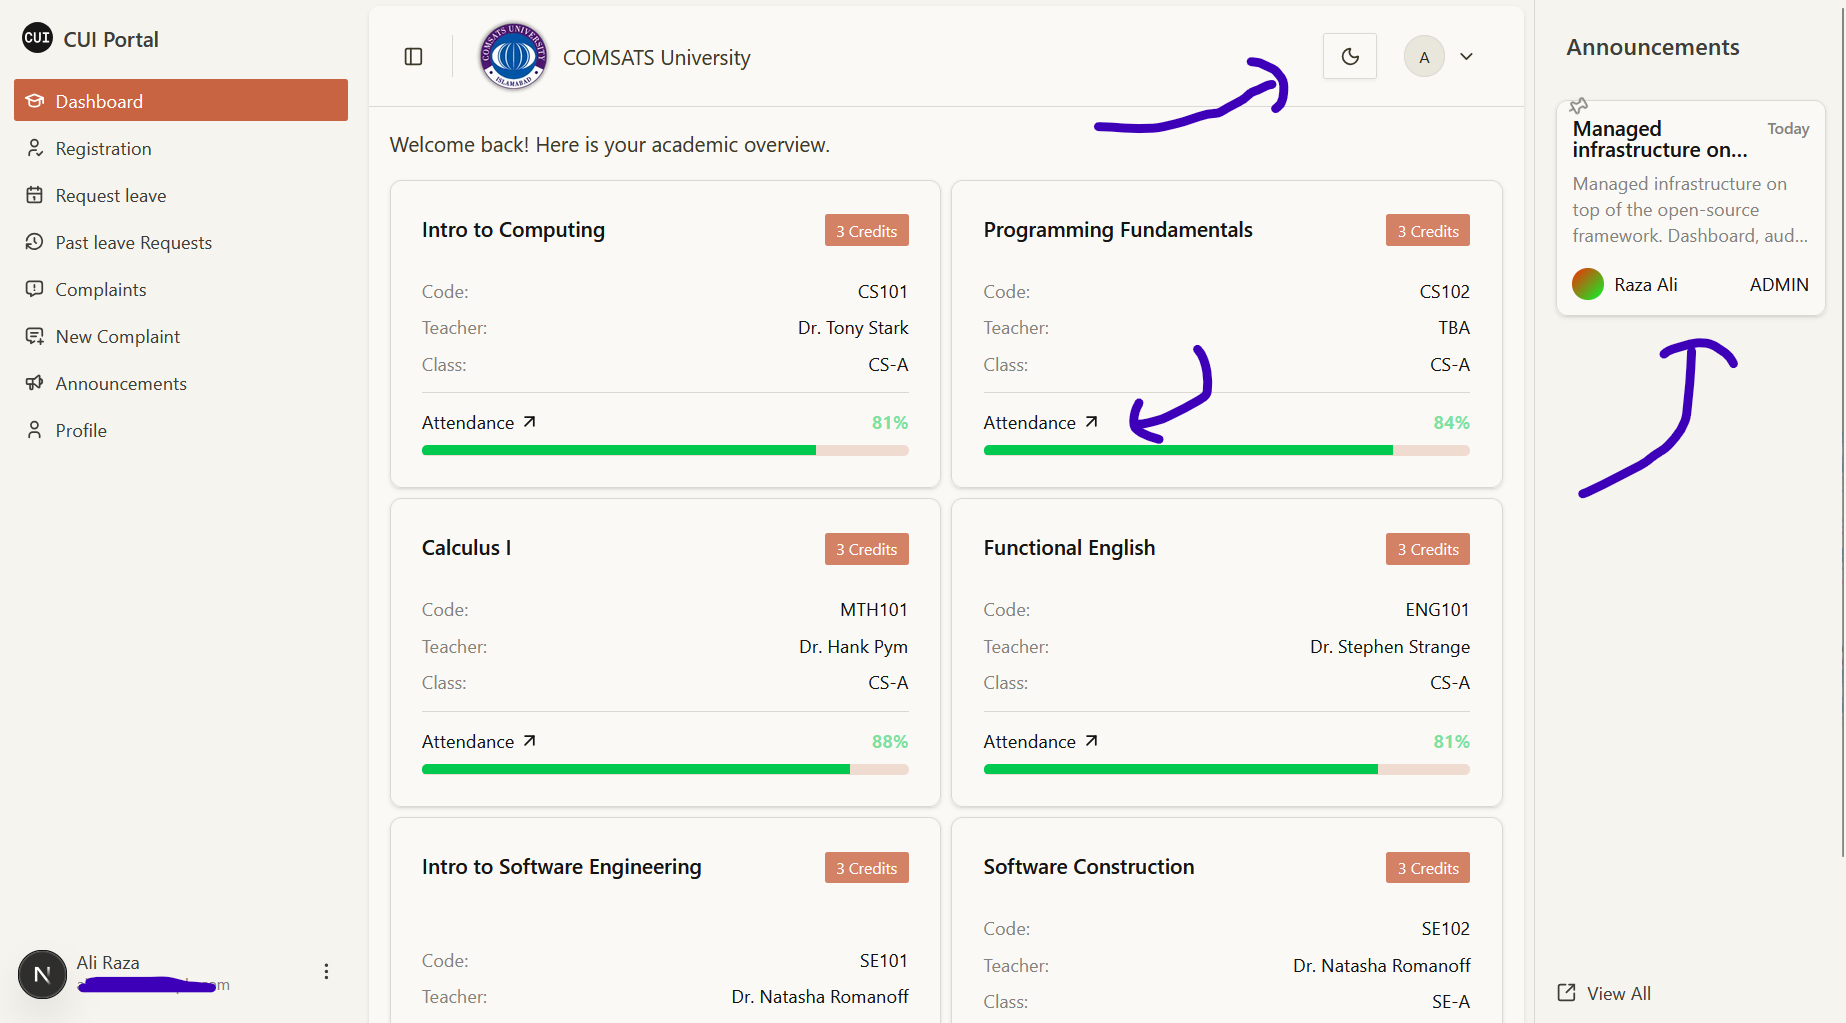
\includegraphics[width=\linewidth]{Figures/web/st-das.png}
  \smallskip
  \textbf{Figure X:} student Dashboard Screen.
\end{center}

% \begin{figure}[h]
% \centering
% \includegraphics[width=0.8\textwidth]{Figures/dashboard_screen.png}
% \caption{Dashboard Screen}
% \end{figure}

% -------------------------------------------------

\subsubsection{Screen 3: Student Leave Request Screen}

\textbf{Purpose:}
This screen enables an authenticated student to submit a formal leave request for a specific enrolled subject. The request is then forwarded to their respective Department Batch Advisor for further review.

\textbf{Components:} \begin{itemize} \item \textbf{Text Content:} Page title (``New Leave Request'') and informational text explaining the purpose of the form. \item \textbf{Navigation Link:} "View all leave Requests" link pointing to the student's leave history. \item \textbf{Form Inputs:} \begin{itemize} \item Subject Selection Dropdown \item Date Picker (Calendar Popover) \item Reason Title Input \item Description Textarea \item Image Evidence Uploader \end{itemize} \item \textbf{Submit Button:} Disables temporarily and shows a loading state ("Submitting...") during the form submission. \end{itemize}

\textbf{Functional Flow:} The user accesses the screen, which dynamically loads their currently enrolled subjects. They fill out the form by picking a subject, selecting a valid date, providing a title and detailed reason, and selectively attaching an image (e.g., a medical certificate). When the user clicks "Submit Leave Request", the system attempts to send the request. If successful, the form is cleared, the page is refreshed to sync the latest state, and a success toast notification appears. If an error occurs, an error toast is displayed.

\textbf{Backend Integration:} Before rendering the screen, Server-Side logic enforces route authorization via \texttt{requirePermission({ leaveRequest: ["create"] })}. If unauthorized, the user is redirected. Once authorized, \texttt{getStudentEnrolledSubjects()} retrieves the necessary data. Upon form submission, the client-side form triggers a Next.js Server Action named \texttt{sendLeaveRequest}. The call runs non-blockingly using React's \texttt{useTransition}.

\textbf{Validation:} Client-side validation is primarily handled via \texttt{react-hook-form} and Zod (\texttt{leaveRequestSchema}) which shows errors as user types.
Specific field constraints include: \begin{itemize} \item \textbf{Date Restrictions:} The Date Picker dynamically disables dates that are in the past, dates that are more than 4 days in the future, and weekends (Saturdays and Sundays). \item \textbf{General Validation:} Form shows errors as user types for title and description \end{itemize}

\begin{center}
  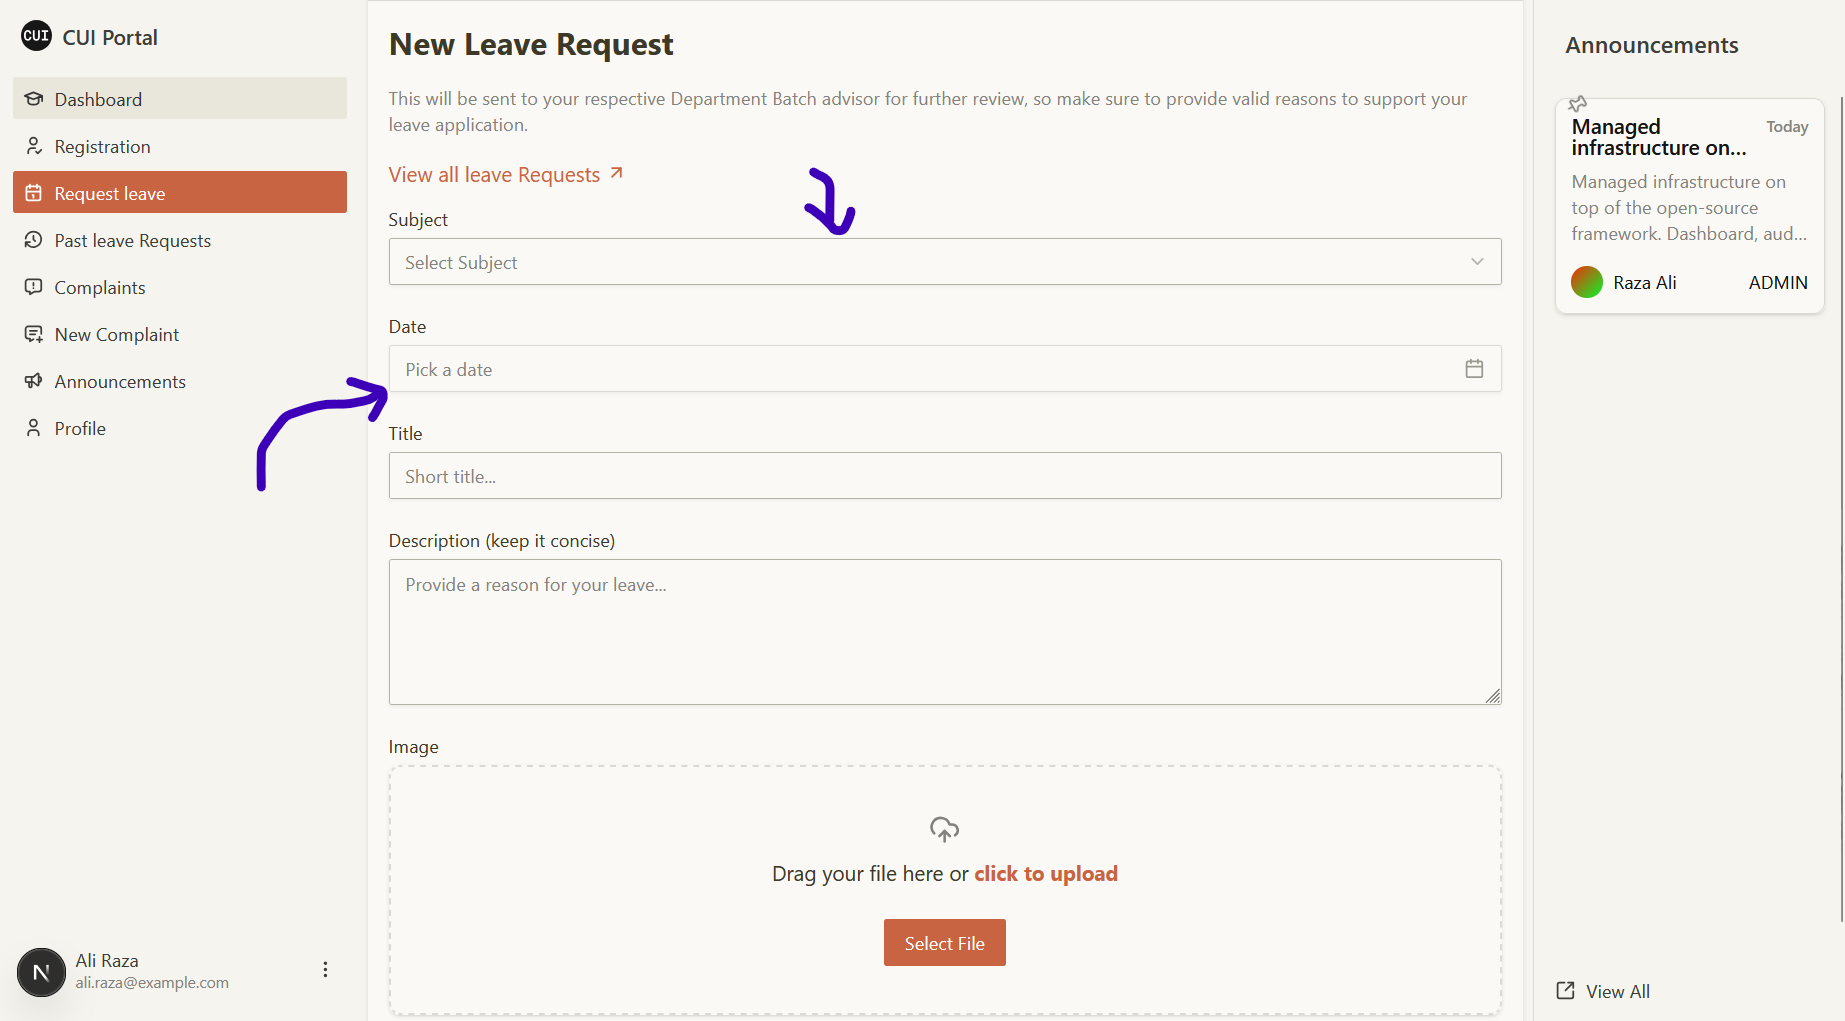
\includegraphics[width=\linewidth]{Figures/web/st-LR.png}
  \smallskip
  \textbf{Figure X:} student leave request Screen.
\end{center}

% -------------------------------------------------

\subsubsection{Screen 4: Student New Complaint Screen}

\textbf{Purpose:}
This screen provides an interface for students to submit new complaints regarding various issues (e.g., academic, administrative). Submitted complaints are forwarded to the respective department's BA for review and resolution.

\textbf{Components:} \begin{itemize} \item \textbf{Header:} Title ("New Complaint") and helper text explaining the purpose and destination of the complaint. \item \textbf{Complaint Form:} \begin{itemize} \item Title input field \item Details textarea for concise description \item Category dropdown (e.g., ACADEMIC) \item Action Buttons: "Reset" to clear the form and "Submit" to send the complaint. \end{itemize} \end{itemize}

\textbf{Functional Flow:} The user accesses the screen and fills in the necessary details—assigning a title, specifying the complaint details, selecting an appropriate category. The user can click "Reset" at any point to clear their inputs. Upon clicking "Submit", a loading transition starts ("Submiting..."). If the submission is successful, a confirmation toast appears, the form is reset, and the user is redirected back to the main complaints listing page (\texttt{/student/complaints}). If an error occurs, an error toast notifies the user.

\textbf{Backend Integration:} The form uses a Next.js Server Action named \texttt{CreateComplaint}. This action handles the secure processing of the complaint data on the server. The submission process is wrapped in React's \texttt{useTransition} hook to manage the pending UI state and a \texttt{tryCatch} utility to gracefully handle any server-side exceptions or API failures without unmounting the form.

\textbf{Validation:} Client-side validation is enforced using \texttt{react-hook-form} paired with Zod validation (\texttt{complaintSchema}). The form validates inputs \texttt{onChange}. If a validation happens (e.g., missing title or details, exceeding length limits), the UI responds immediately by setting the ARIA invalid state on the related input and showing error messages below the field component.

\begin{center}
  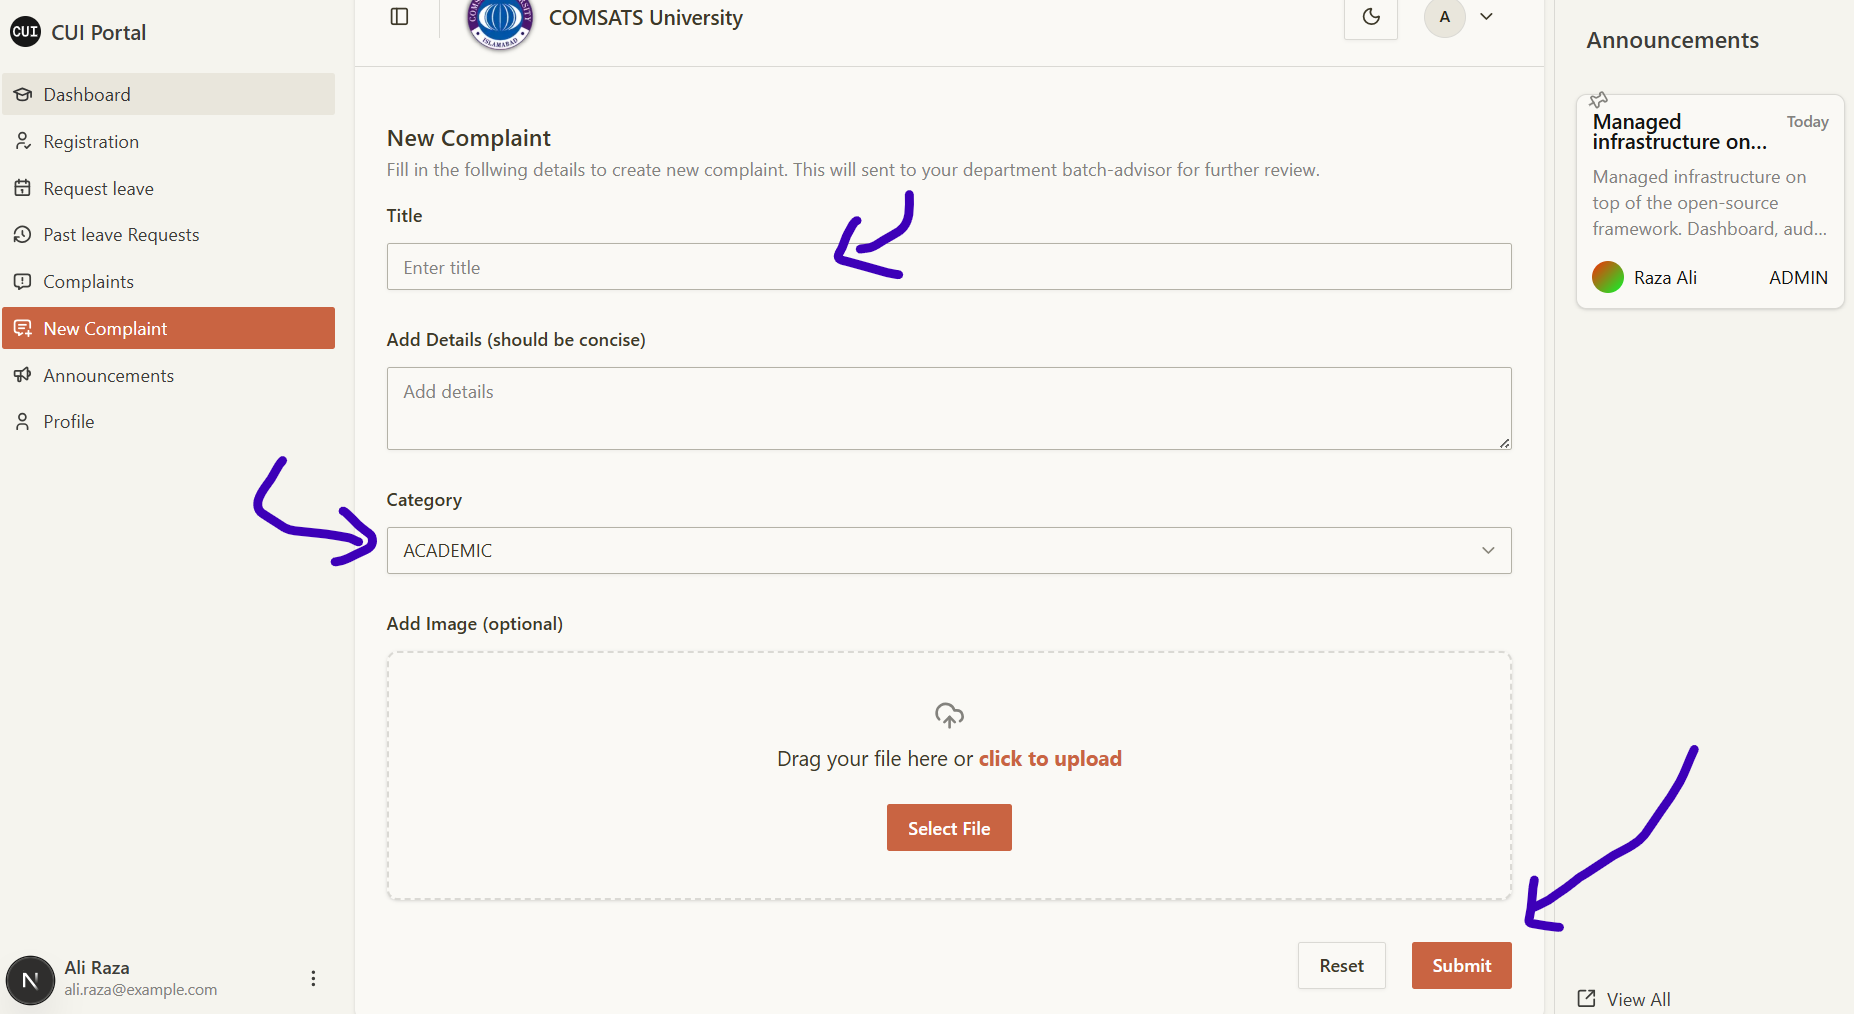
\includegraphics[width=\linewidth]{Figures/web/st-comp-new.png}
  \smallskip
  \textbf{Figure X:} student new complaint Screen.
\end{center}

% -------------------------------------------------

\subsubsection{Screen 5: Professor Attendance Screen}

\textbf{Purpose:}
This screen enables professors to manage and record the attendance for a specific class offering. It allows bulk marking of attendance and provides the ability to specify the lecture's topic, date, and duration. Professor can see leave request from students with their status.

\textbf{Components:} \begin{itemize} \item \textbf{Header:} Title ("Manage attendance for class") \item \textbf{Lecture Details Form:} \begin{itemize} \item Topic input field \item Date picker (Calendar popover) \item Start Time and End Time selectors (Popover dropdowns) \end{itemize} \item \textbf{Attendance Table:} \begin{itemize} \item Bulk Selection Header (Count of students and selected students) \item Bulk Action Buttons ("Mark as Present", "Mark as Absent") \item Student Rows (Image, Name with optional Leave Request indicator, Registration Number) \item Individual Attendance Radio buttons (Present/Absent for each student) \end{itemize} \item \textbf{Action Button:} "Mark Attendance" button to submit the form. \end{itemize}

\textbf{Functional Flow:} The professor arrives at the screen which loads the roster for the assigned class securely from the server. They enter the lecture details: topic, date (automatically disabled for future dates or weekends), start time, and end time.

For attendance, the default state for all students is "Absent". The professor can mark attendance individually using radio buttons per student, or use checkboxes to select multiple students and apply a bulk status via the "Mark as Present" or "Mark as Absent" buttons above the table. If a student has a pending leave request, a blinking alert icon appears next to their name, which opens a dialog detailing the request's date and reason, with a link to view full details.

Upon clicking "Mark Attendance", the client initiates a server action transition. If successful, a toast notification confirms submission, the form's lecture topic is cleared, and the attendance states revert to the default (Absent).

\textbf{Backend Integration:} The initial student list is fetched asynchronously via the \texttt{getProfessorSectionStudents({ offeringId })} function on the server side before the page fully renders. The page leverages a \texttt{Suspense} boundary to display a skeleton loader while this data is fetching. Form submission utilizes a Next.js Server Action named \texttt{markAttendance}. The action executes safely via a \texttt{tryCatch} utility, running inside a React \texttt{useTransition} hook to maintain UI responsiveness without a page reload.

\textbf{Validation:} The \texttt{AttendanceForm} uses \texttt{react-hook-form} with a Zod resolver (\texttt{attendanceFormSchema}). \begin{itemize} \item \textbf{Date Validation:} The date picker restricts selection to the current date or past dates, filtering out weekends. Manually selecting an invalid date updates the field error state instantly. \item \textbf{Time Validation:} The logic prevents selecting an 'End Time' that is the identical block as the 'Start Time'. \item \textbf{General Validation:} Any failed constraints during submission trigger inline field errors or global error toasts. \end{itemize}

\begin{center}
  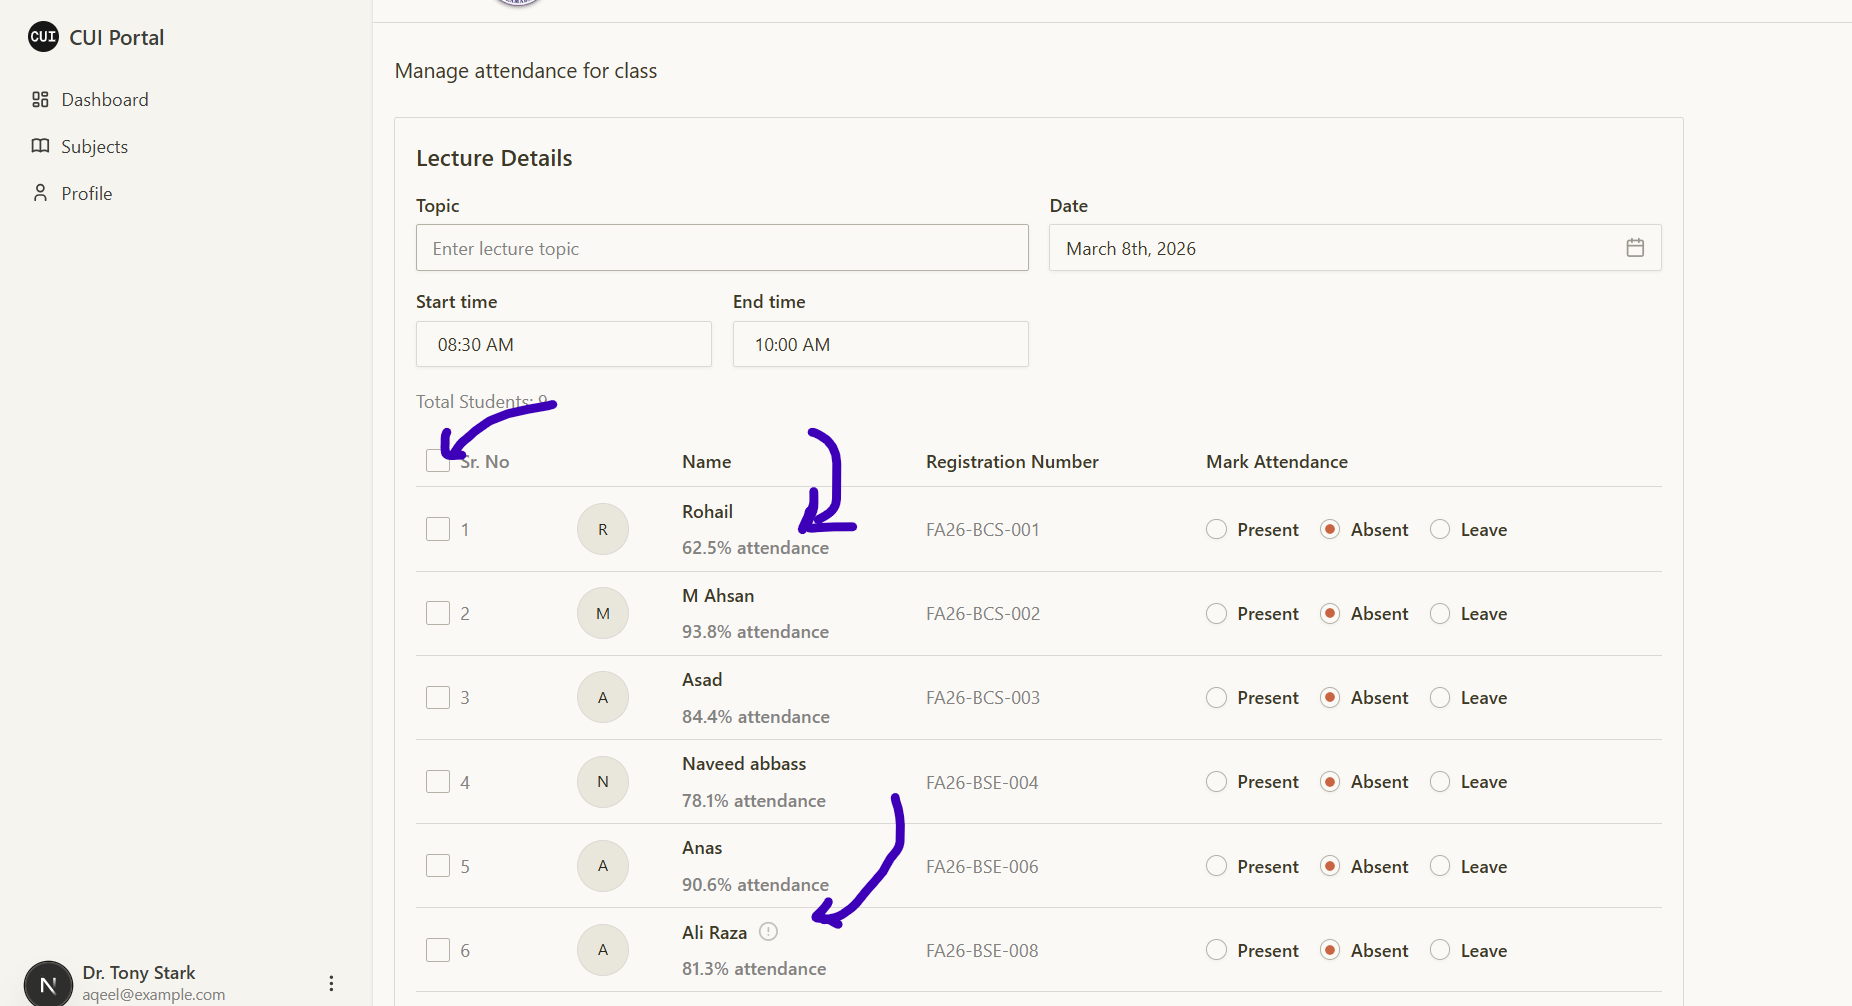
\includegraphics[width=\linewidth]{Figures/web/prf-att.png}
  \smallskip
  \textbf{Figure X:} Proffessor attendance Screen.
\end{center}

% -------------------------------------------------

\subsubsection{Screen 6: Batch Advisor Complaints Screen}

\textbf{Purpose:}
This screen provides Batch Advisors with a centralized dashboard to view, manage, and process complaints submitted by students within their assigned batch.

\textbf{Components:}
\begin{itemize}
    \item \textbf{Header:} Page title ("Batch Advisor Complaints") and a brief description.
    \item \textbf{Filter and Search Bar:}
    \begin{itemize} \item Global text search input (searches across title, details, and student names) \item Dropdown filters for Status, Attachment presence, and Category \item Date Range picker (Calendar popover) \item "Clear Filters" button (conditionally rendered when filters are active) \end{itemize} \item \textbf{Complaints Data Table:} \begin{itemize} \item Draggable column headers for customizable row ordering via drag-and-drop \item Data columns: Serial Number, Student (Name + Registration No), Title (truncated), Category, Status (badge styling), Created Date, Attachment status, and Actions \item "No complaints found" empty state \end{itemize} \item \textbf{Pagination Controls:} \begin{itemize} \item Rows per page selector \item Current result range indicator (e.g., "1-10 of 50") \item Navigation buttons (First, Previous, Next, Last) \end{itemize} \end{itemize}

\textbf{Functional Flow:} The Batch Advisor accesses the page to see a paginated list of complaints. They can filter the data using the search bar, dropdowns, or date picker; these interactions dynamically update the URL search parameters to maintain state. The table columns can be reordered by dragging the headers horizontally. Clicking on the "Actions" column allows the advisor to interact with a specific complaint (e.g., view details or change status). The pagination controls at the bottom navigate through large data sets.

\textbf{Backend Integration:} The page uses Next.js server components to fetch data initially. \texttt{baComplaintsSearchParamsCache} from \texttt{nuqs} parses the URL search parameters on the server and passes them to the \texttt{baGetComplaints(params)} data access layer, executing database queries efficiently. For client-side interactions, the \texttt{BaComplaintsTable} utilizes \texttt{nuqs}' \texttt{useQueryStates} to synchronize filter, sort, and pagination states (like \texttt{sortBy}, \texttt{page}, \texttt{status}) with the browser's URL, updating the server-rendered results incrementally.

\textbf{Validation:} Filter variables and pagination inputs are validated and parsed through tightly typed \texttt{nuqs} parsers (\texttt{baComplaintsSearchParamsParsers}) to ensure the backend receives clean, safe parameters (e.g., ensuring page numbers are integers, and categories map to valid \texttt{ComplaintCategory} enums).

\begin{center}
  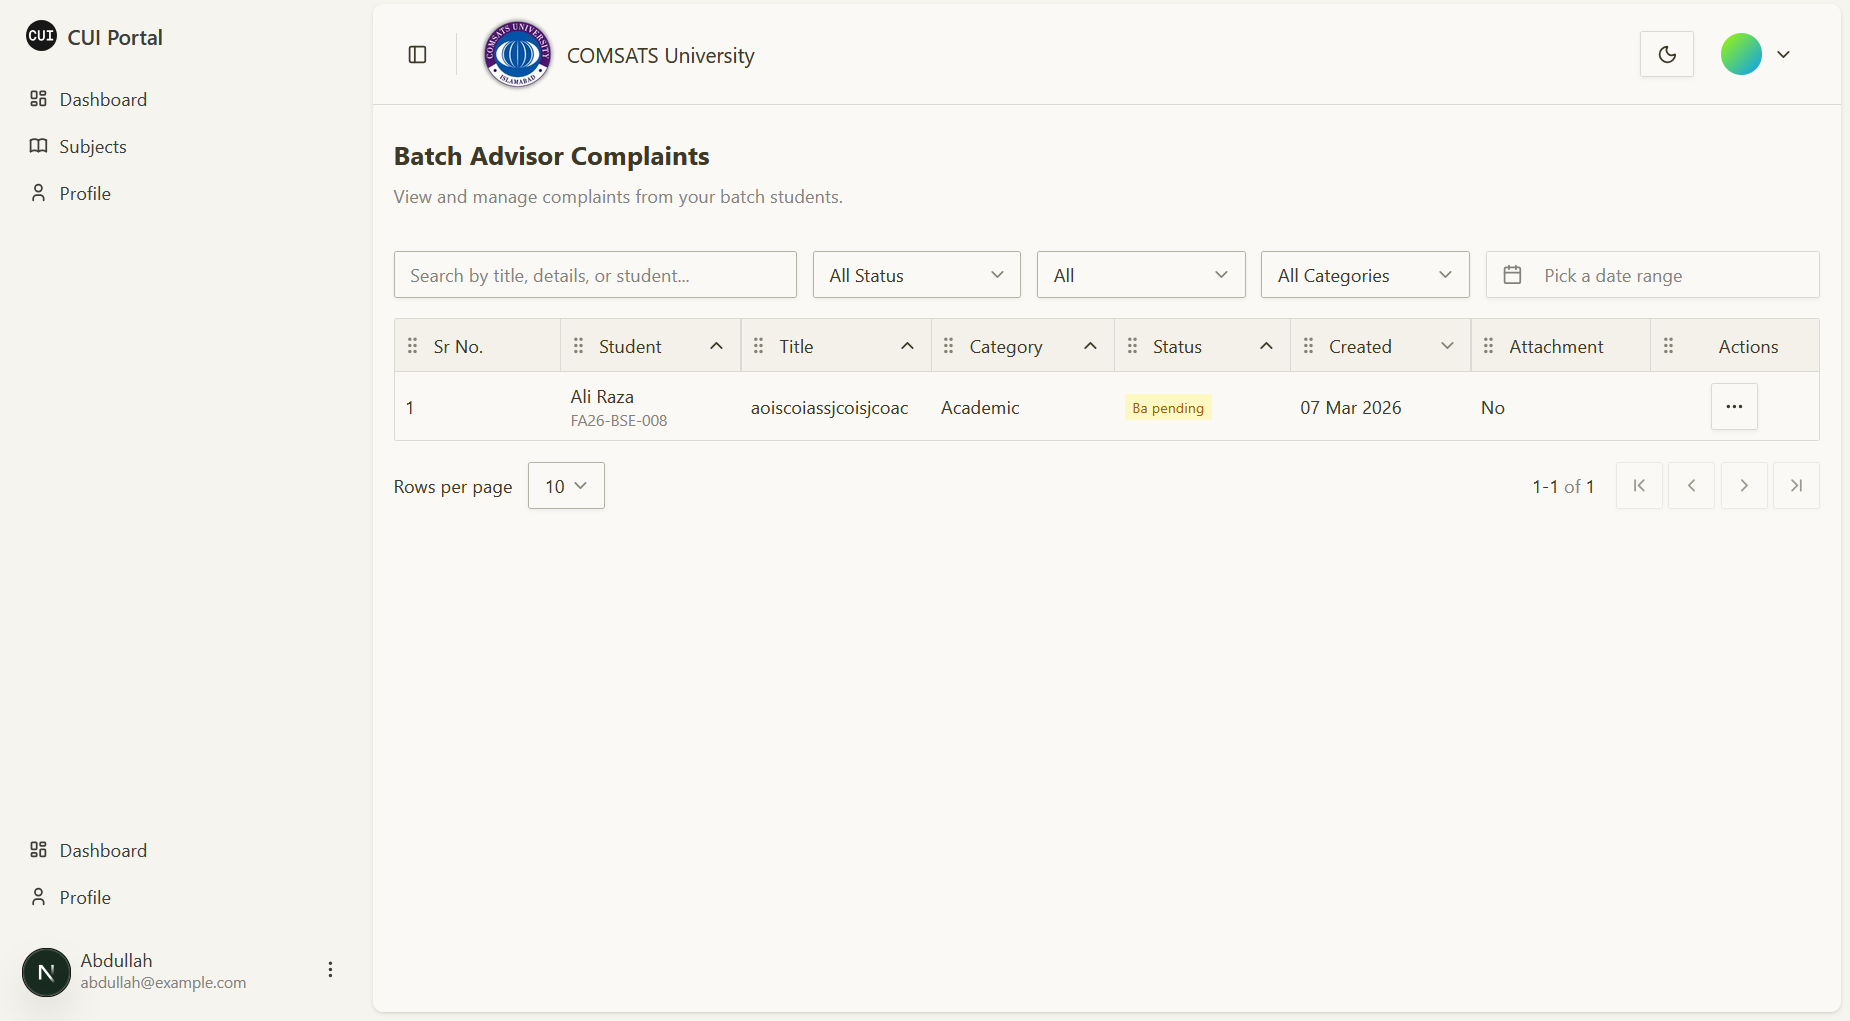
\includegraphics[width=\linewidth]{Figures/web/ba-lr.png}
  \smallskip
  \textbf{Figure X:} BA complaints Screen.
\end{center}

% -------------------------------------------------
% 5.5.3 Navigation Flow Diagram
% -------------------------------------------------

\subsection{Navigation Flow Diagram}

\begin{center}
  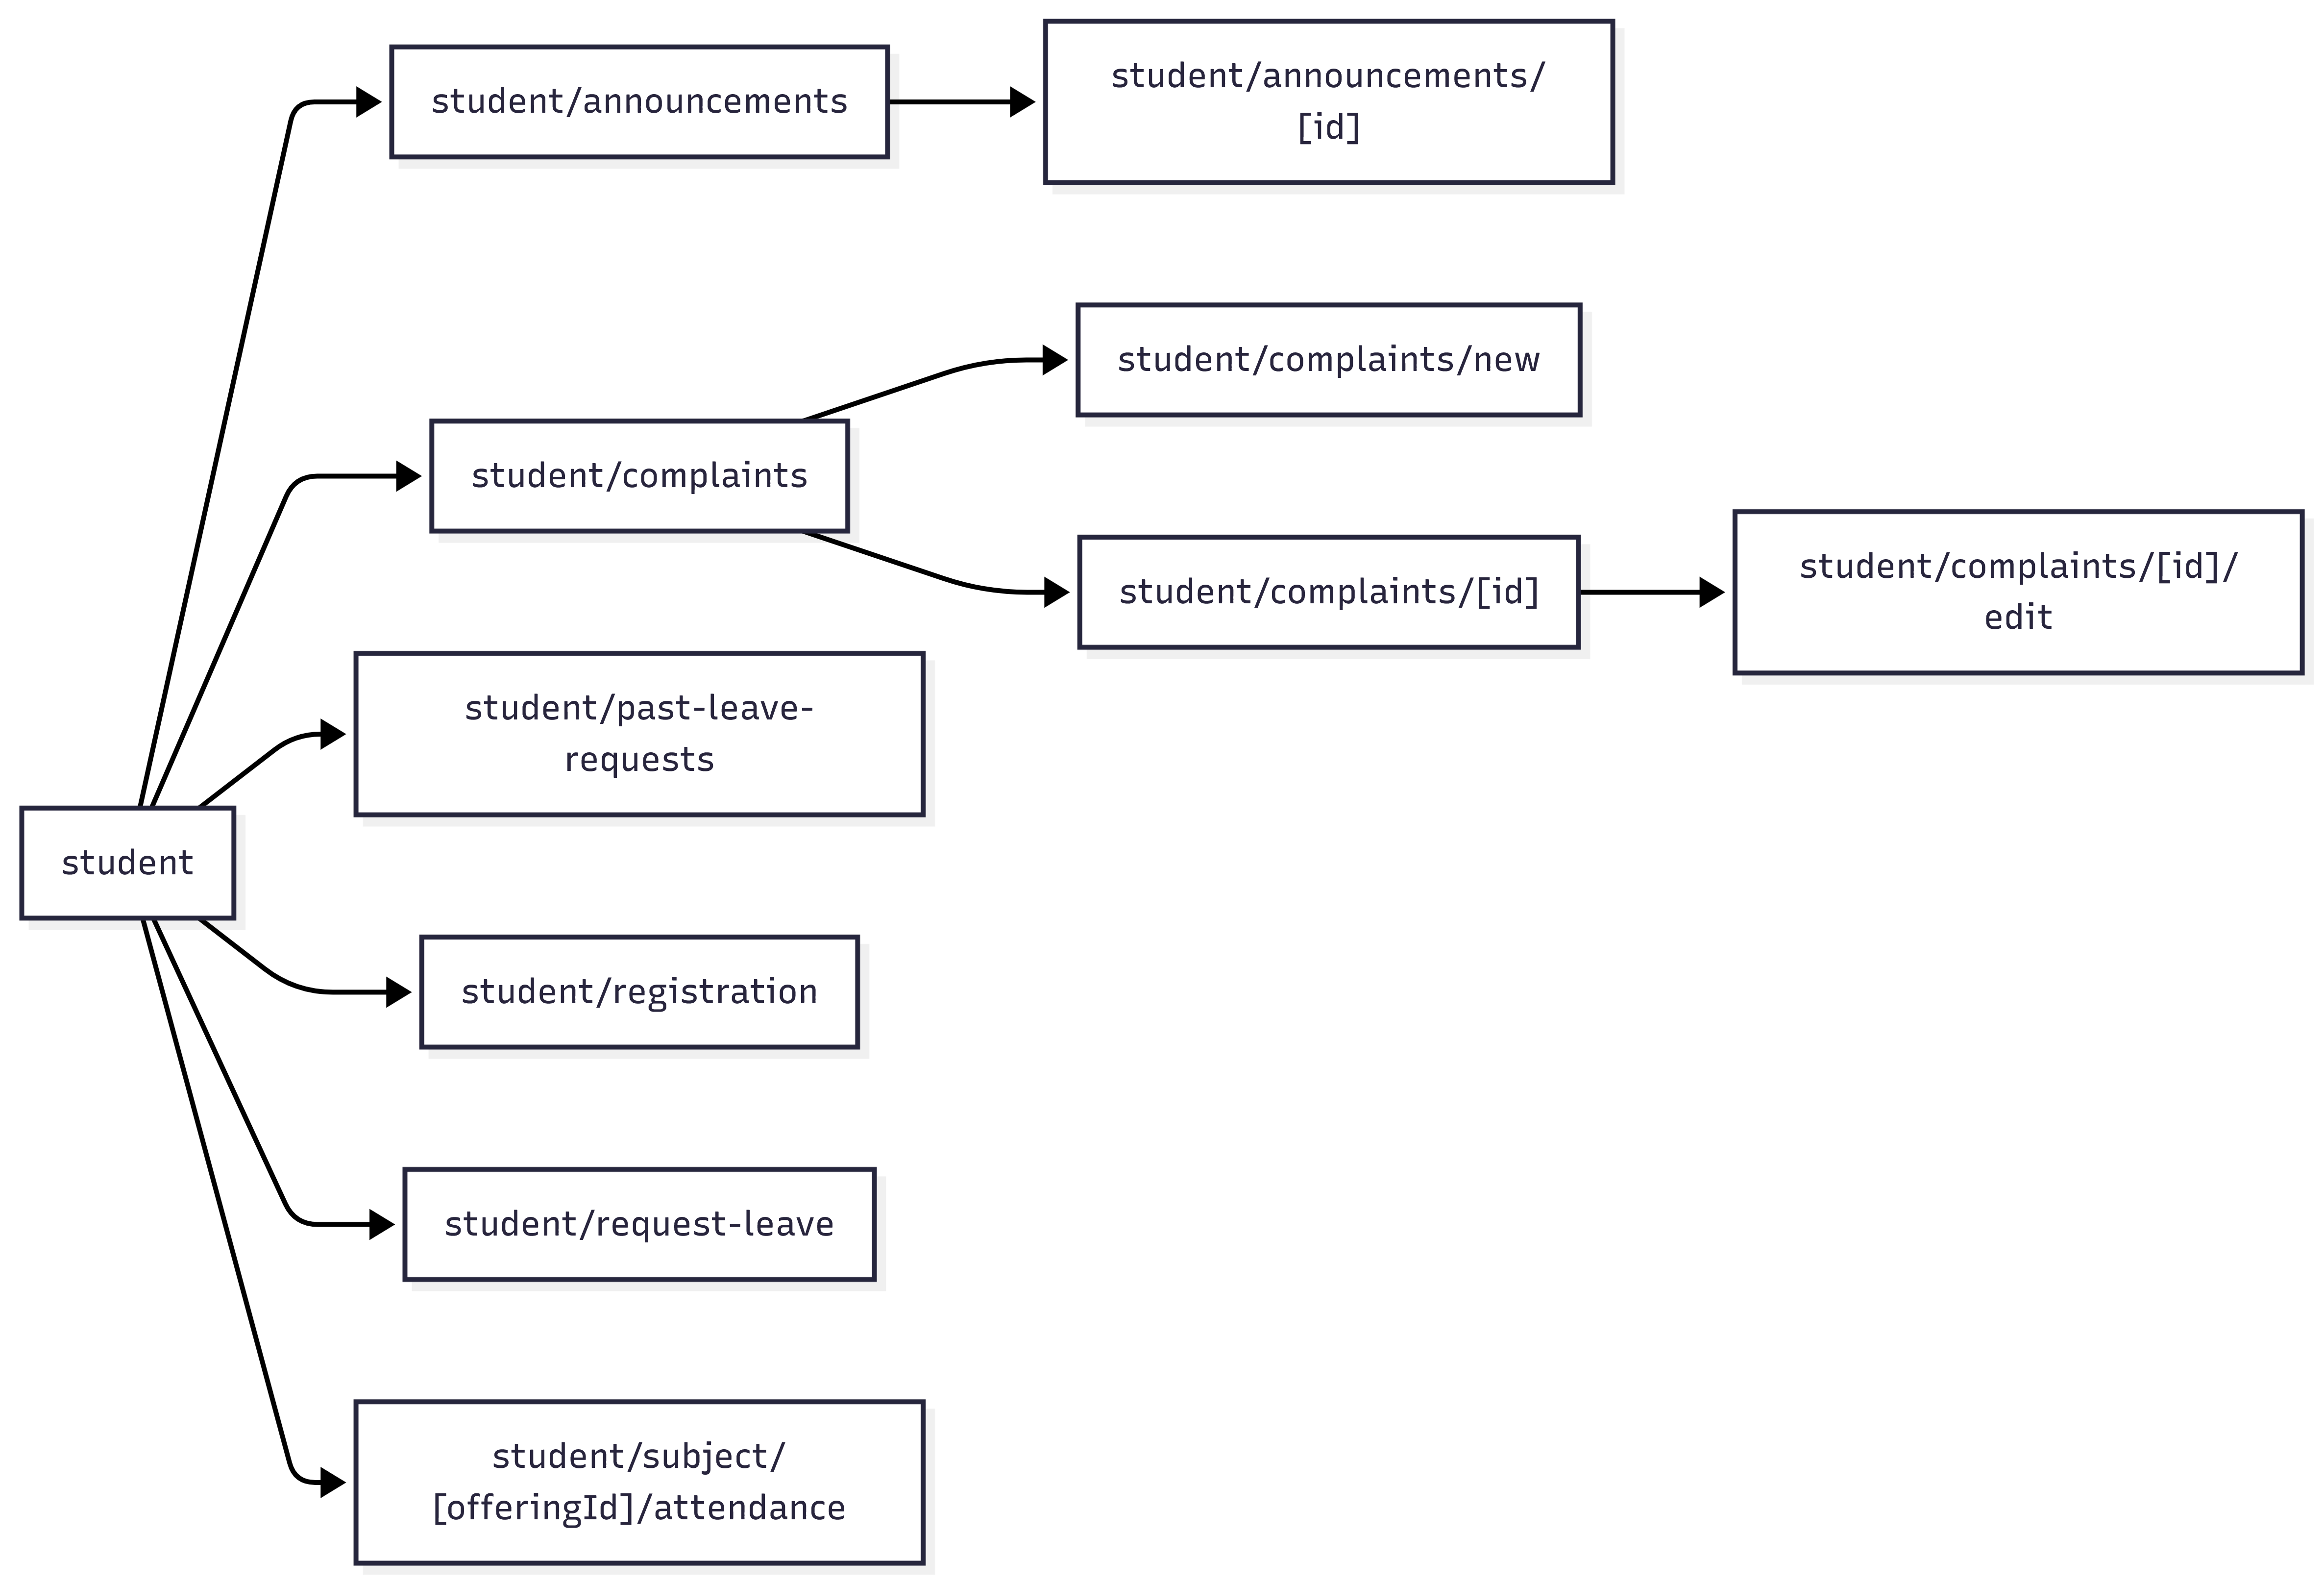
\includegraphics[width=\linewidth]{Figures/flow/st-f.png}
  \smallskip
  \textbf{Figure X:} Student navigation flow.
\end{center}

\begin{center}
  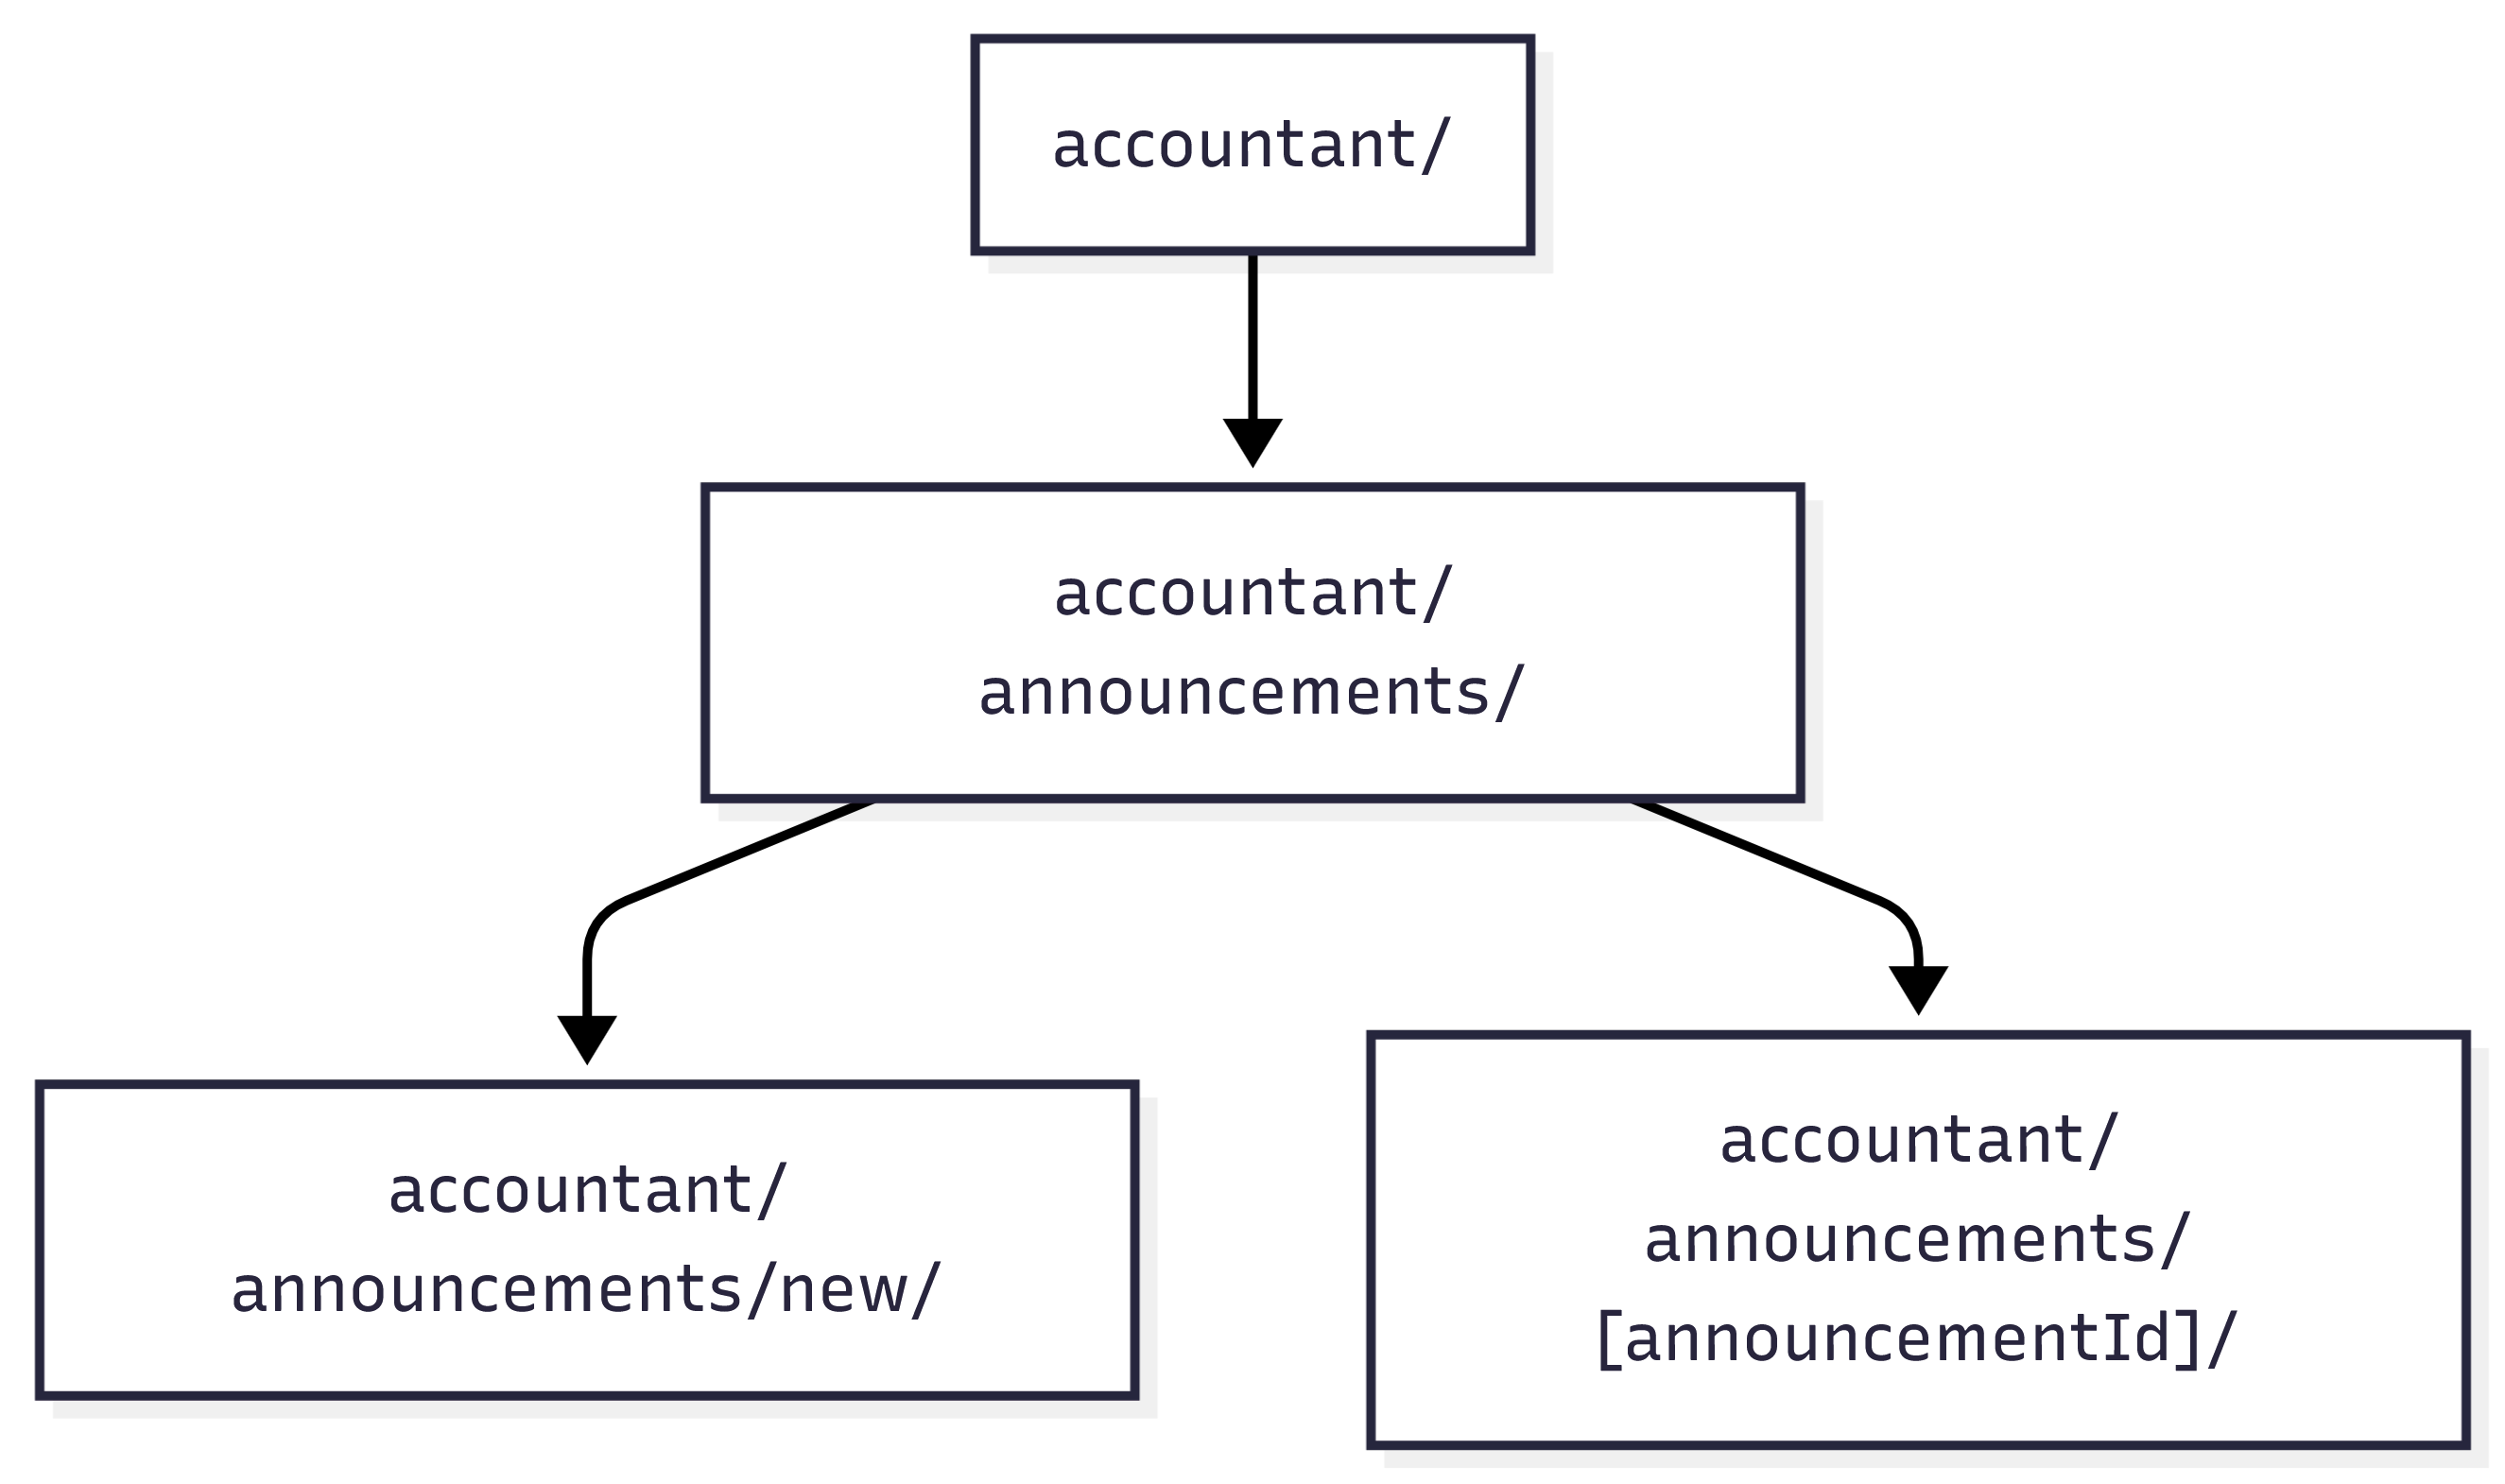
\includegraphics[width=\linewidth]{Figures/flow/acc-f.png}
  \smallskip
  \textbf{Figure X:} Accountant navigation flow.
\end{center}


\begin{center}
  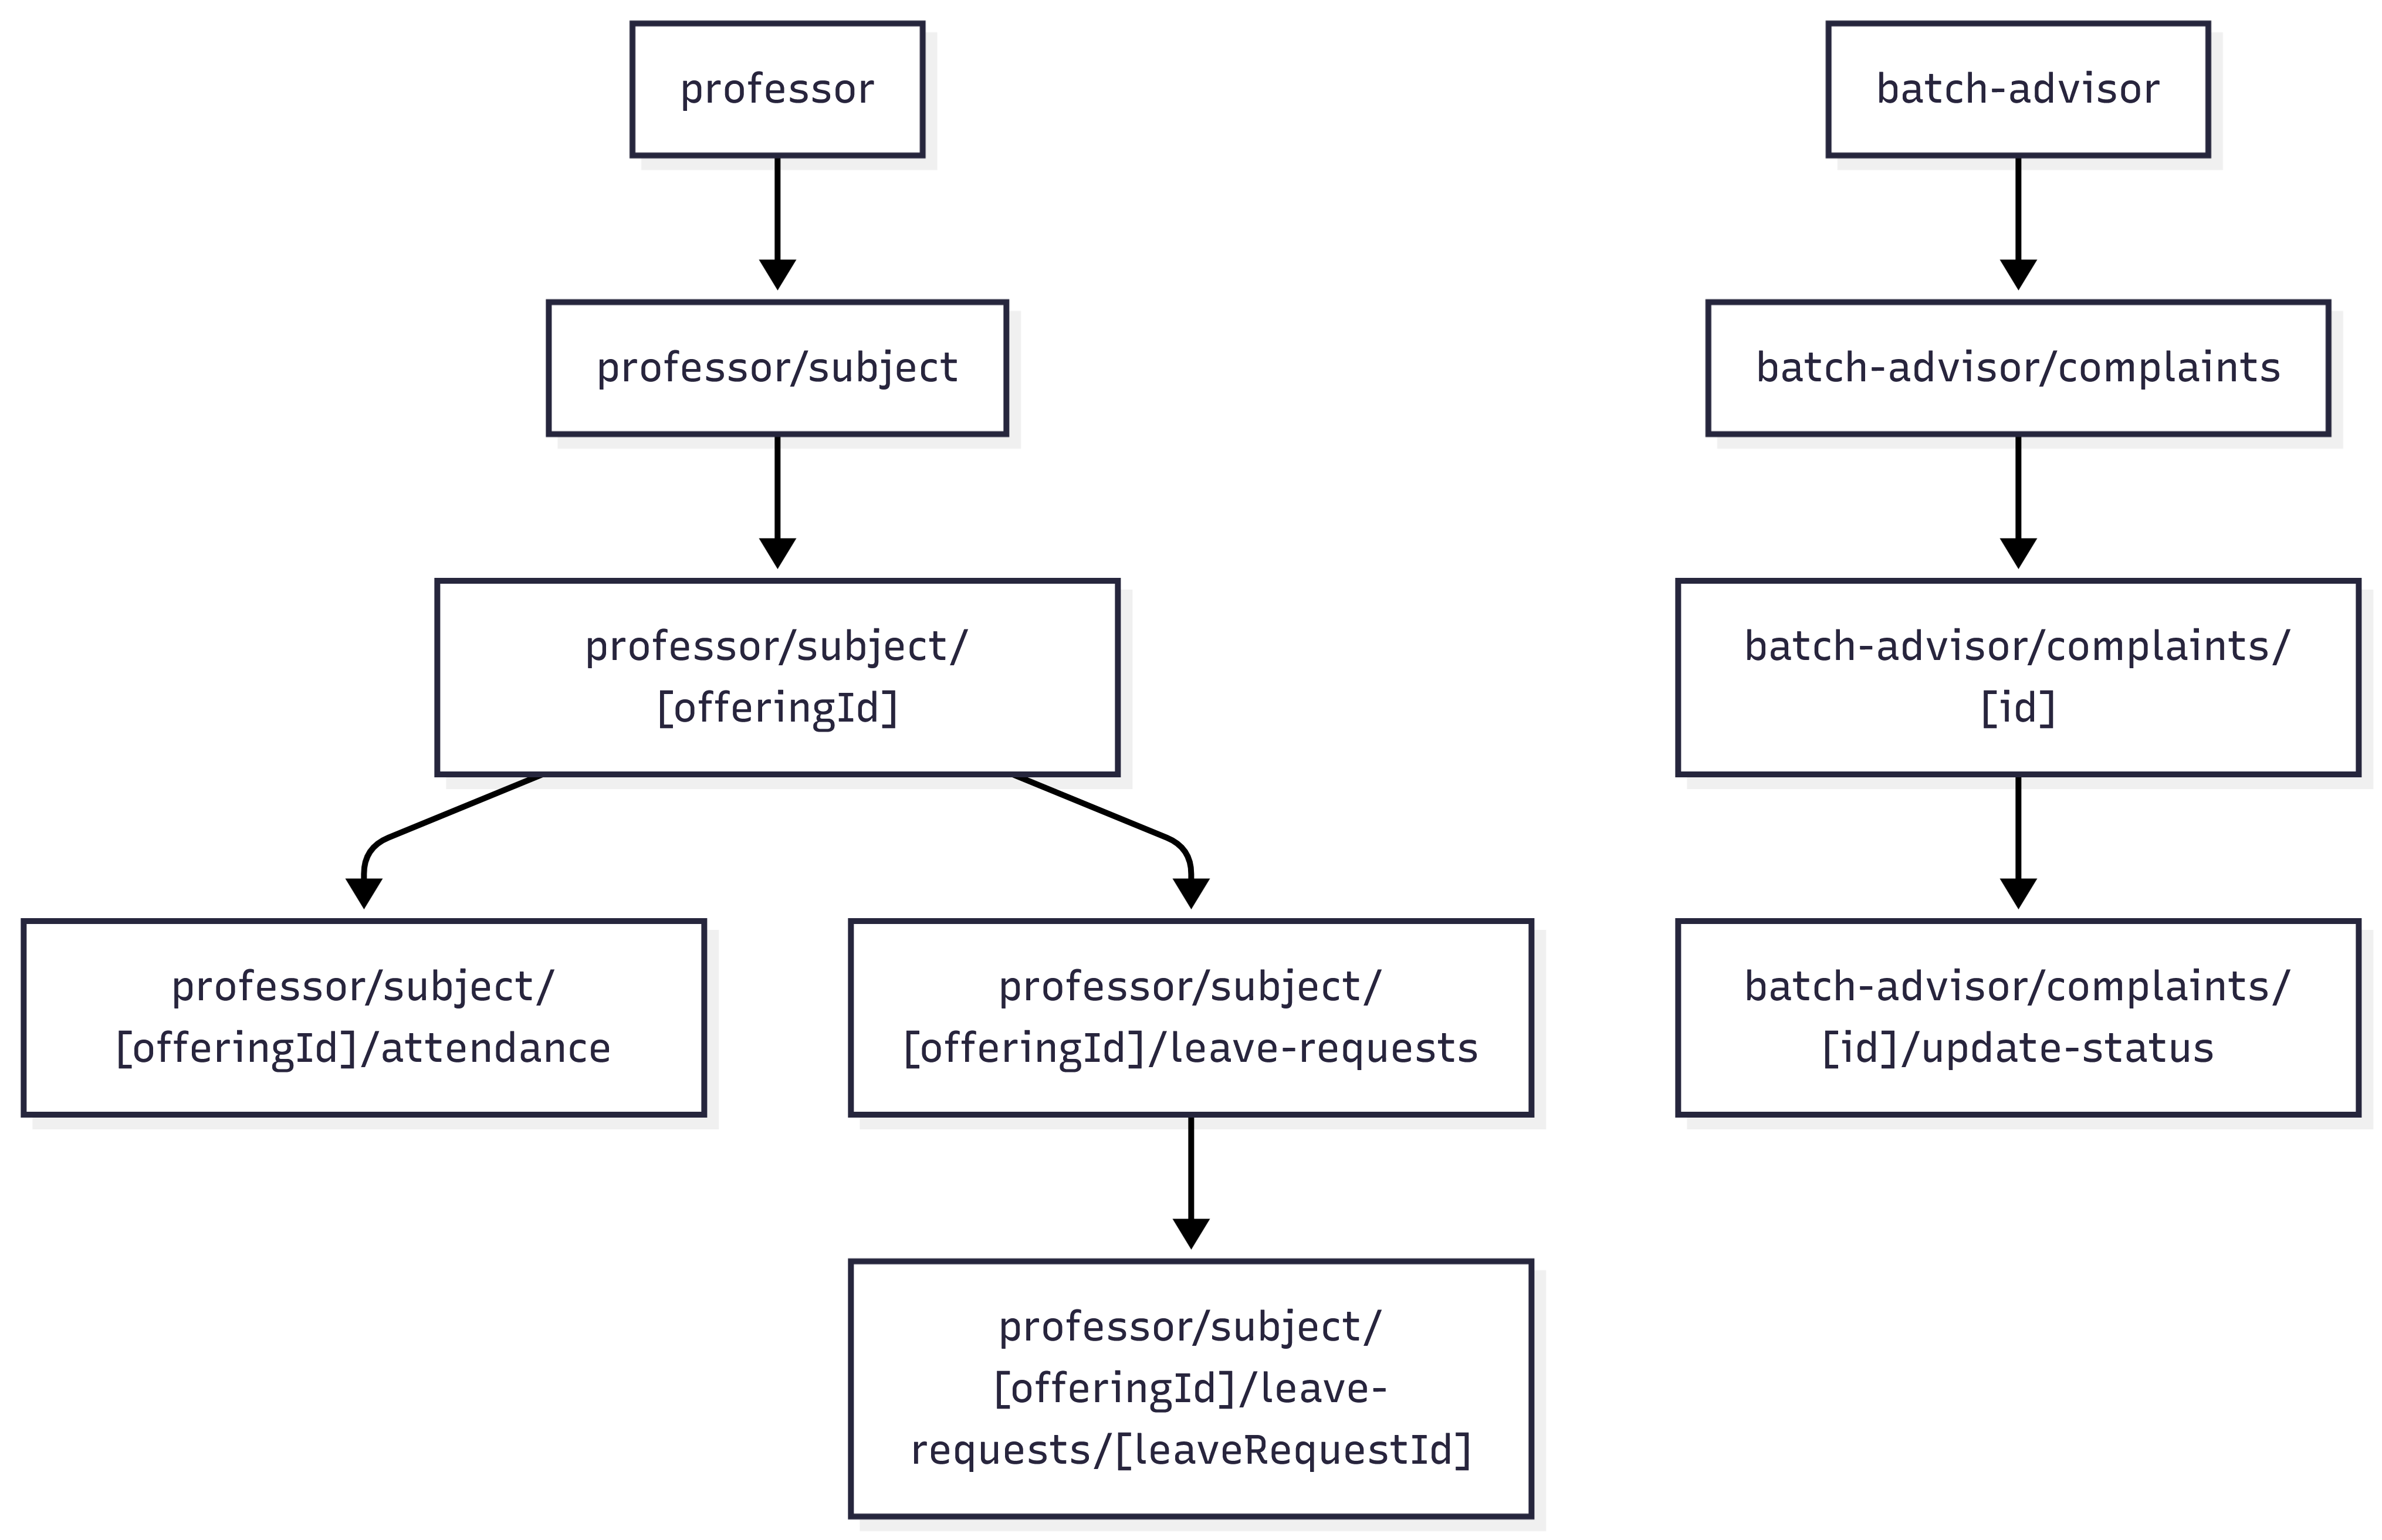
\includegraphics[width=\linewidth]{Figures/flow/prf-f.png}
  \smallskip
  \textbf{Figure X:} Professor navigation flow.
\end{center}

\begin{center}
  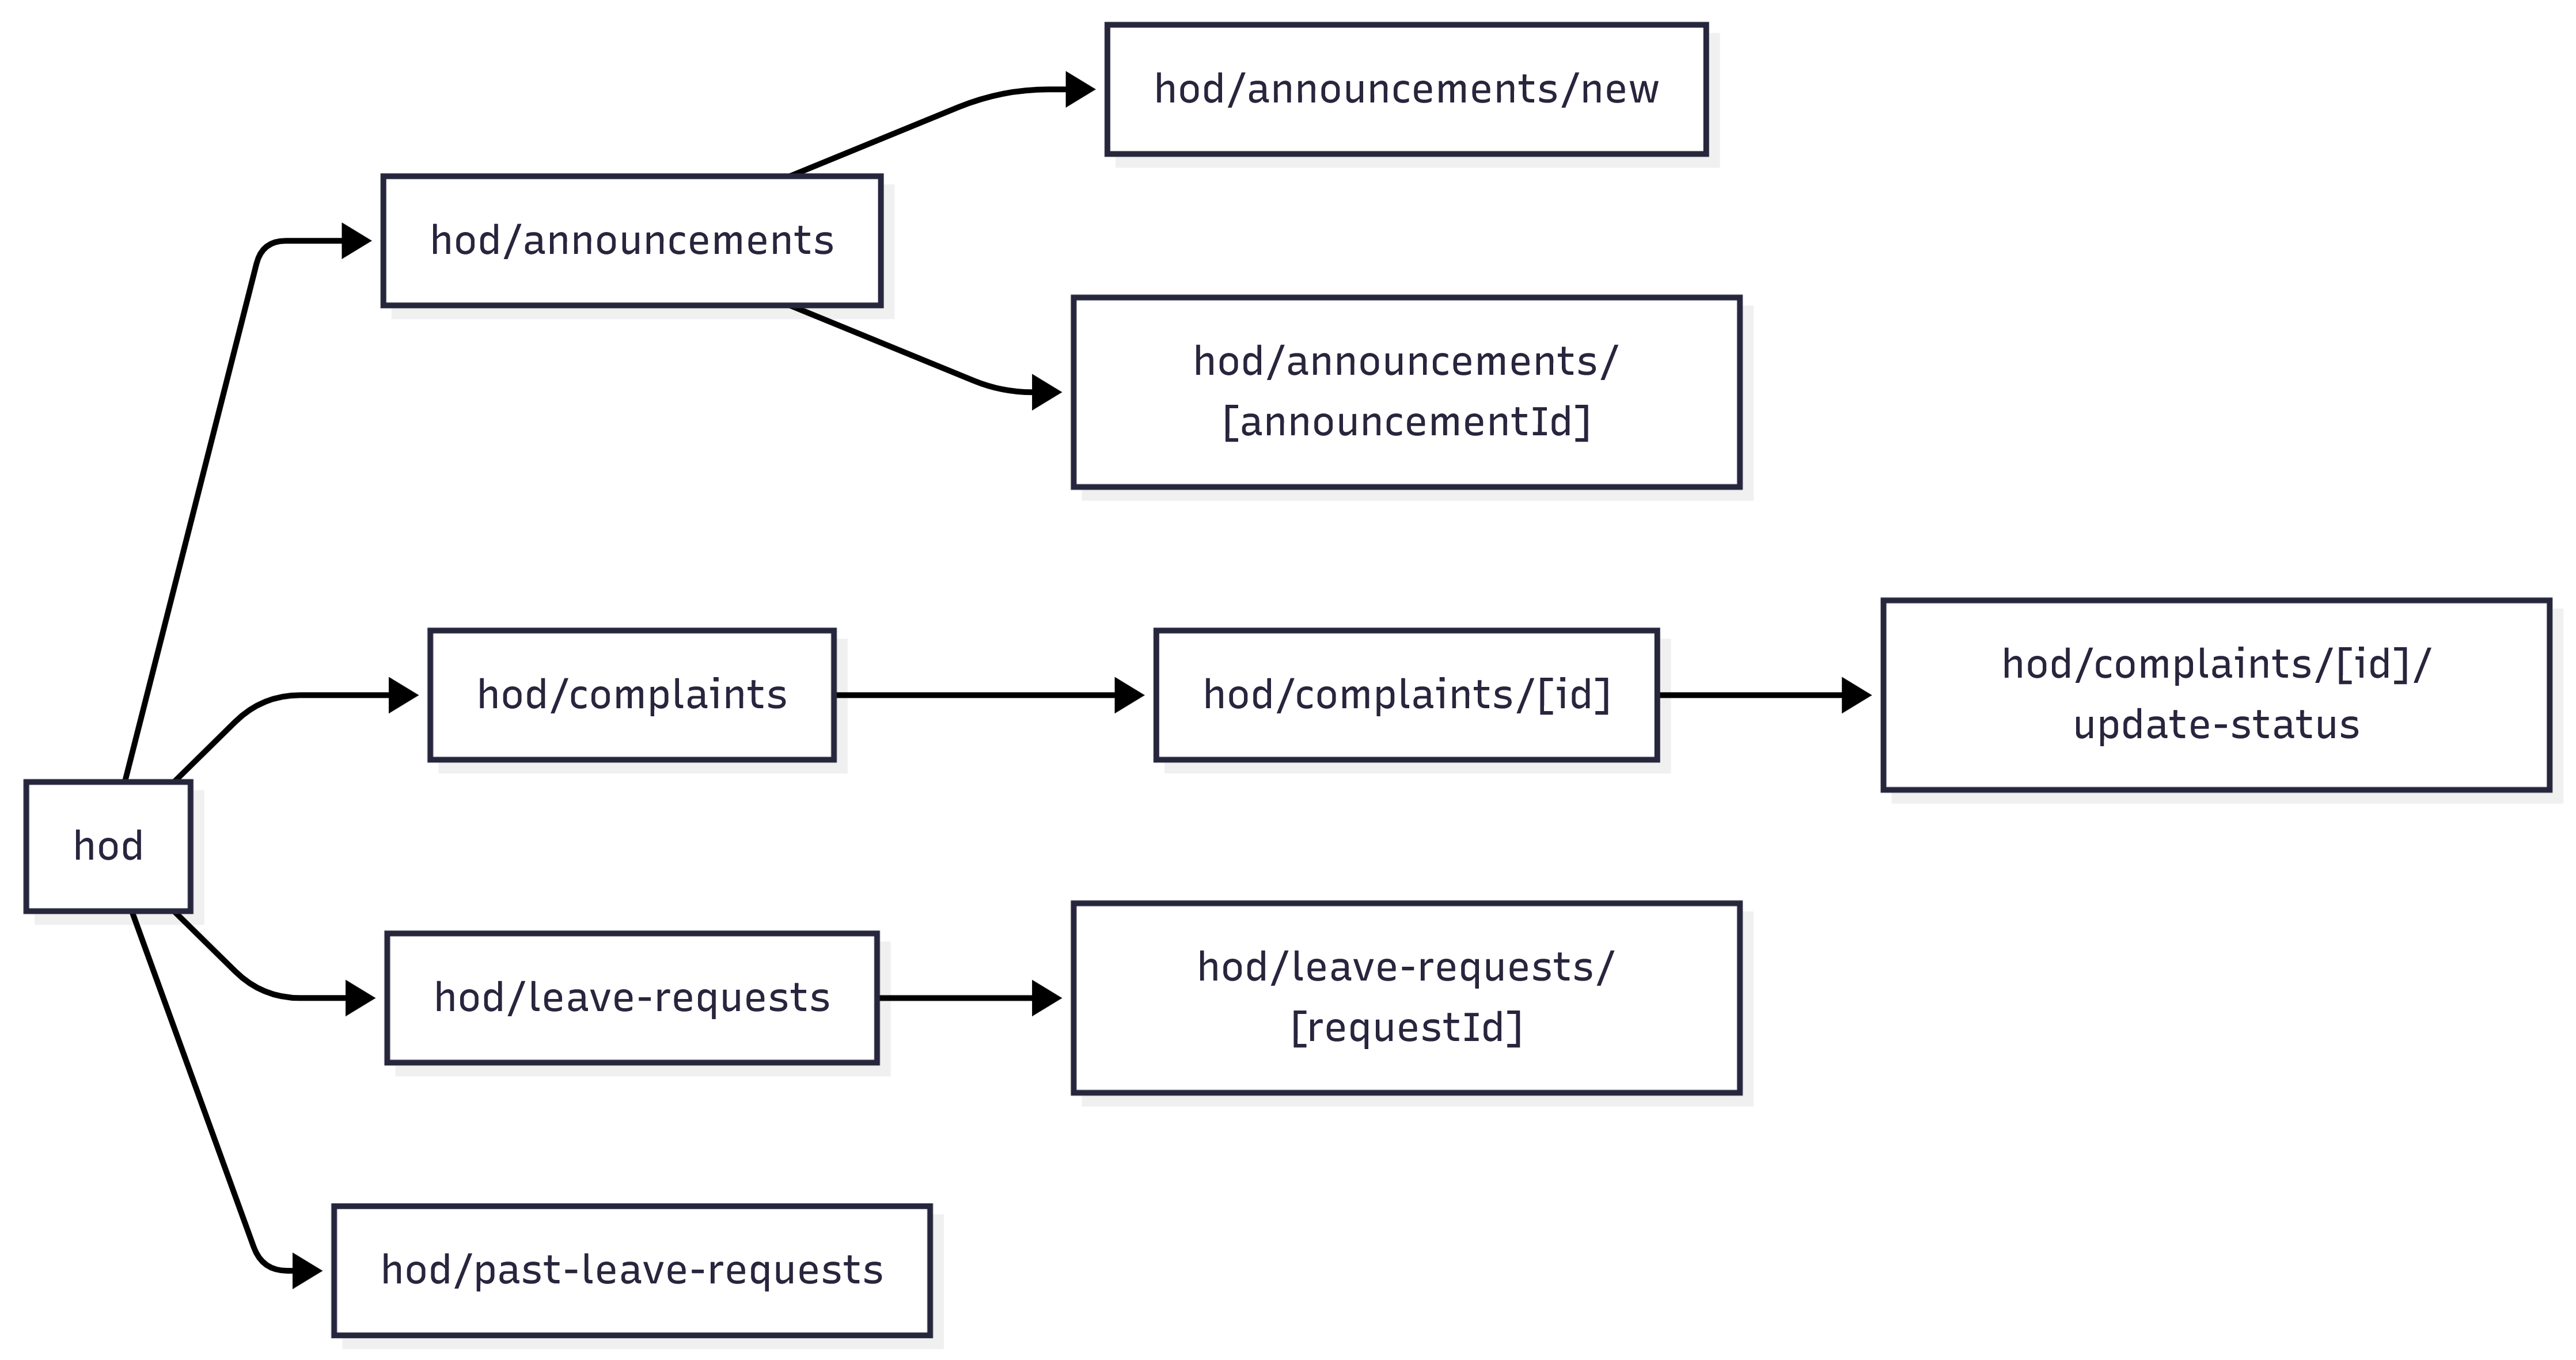
\includegraphics[width=\linewidth]{Figures/flow/hod.png}
  \smallskip
  \textbf{Figure X:} HOD navigation flow.
\end{center}

\begin{center}
  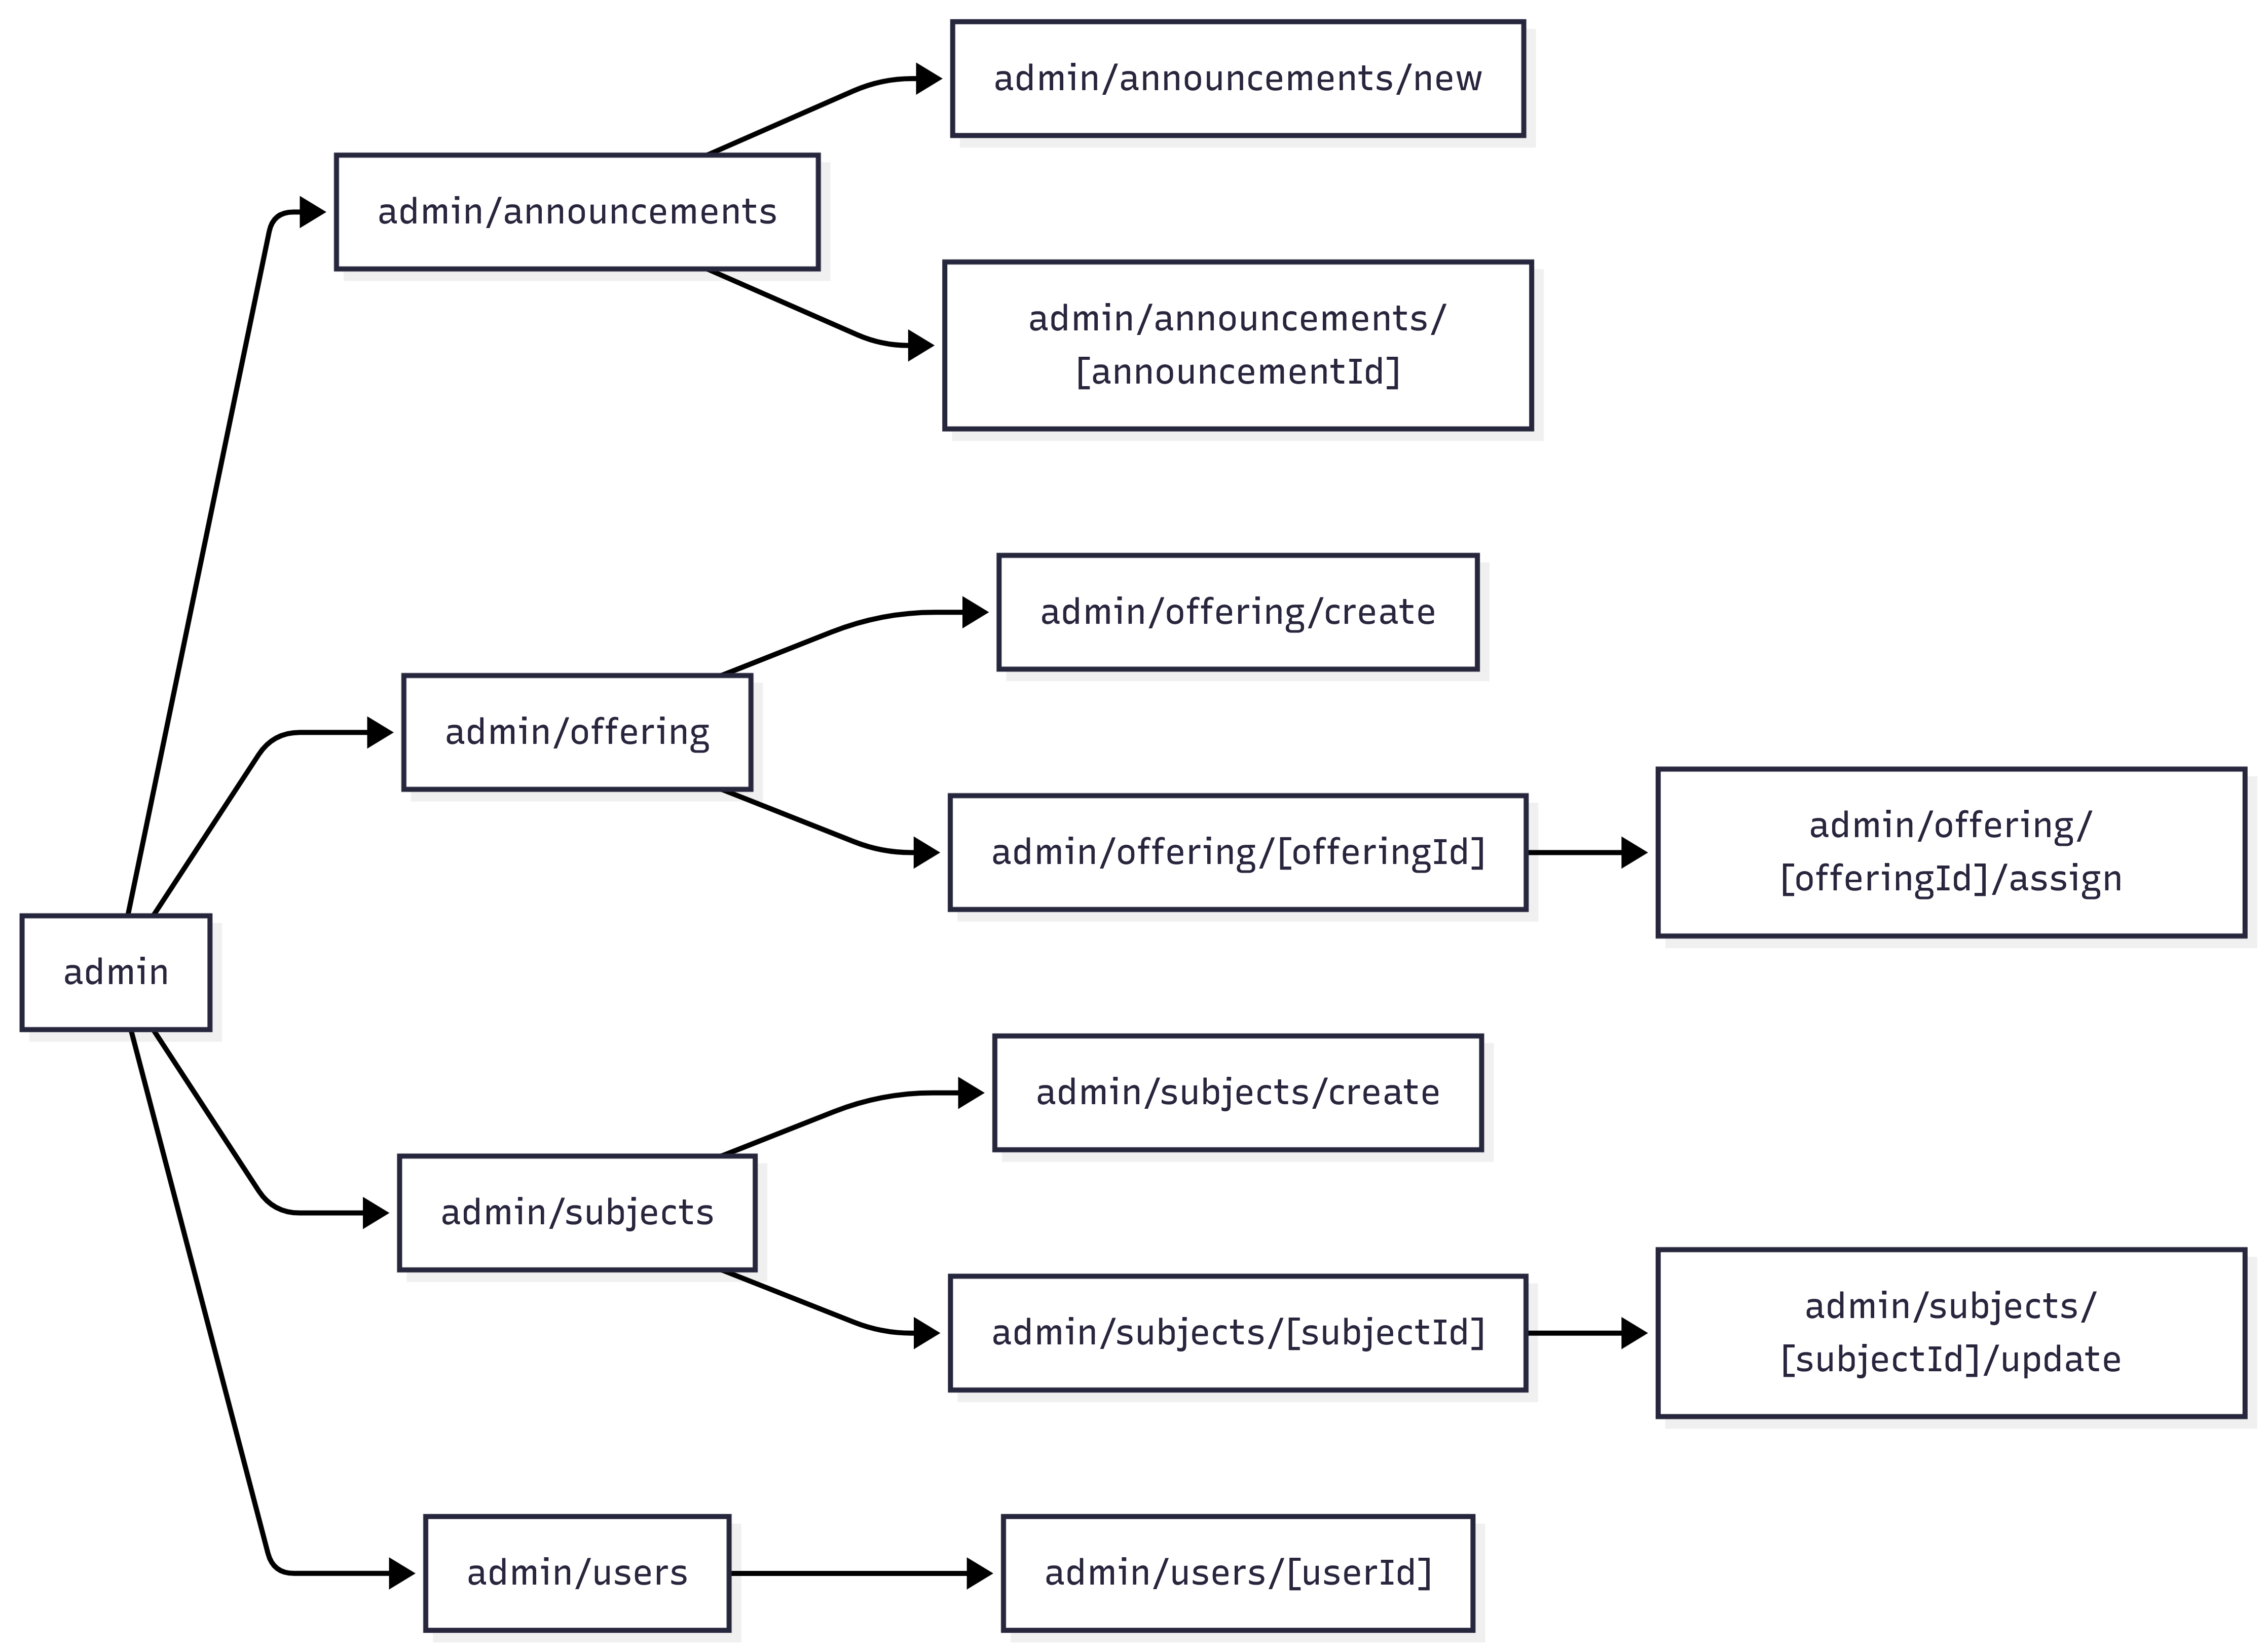
\includegraphics[width=\linewidth]{Figures/flow/admin-f.png}
  \smallskip
  \textbf{Figure X:} Admin navigation flow.
\end{center}

% -------------------------------------------------
% 5.5.4 Responsiveness & Performance
% -------------------------------------------------

\subsection{Responsiveness and Performance}

\textbf{Mobile and desktop adaptibility:}
\begin{itemize}
     
    \item \textbf{Sidebar:}
\begin{itemize}
    \item Large screens (desktop) show sidebar open by default.
    \item On smaller screens (mobile) sidebar is hidden by default and can be toggled using sidebar toggler in header.
\end{itemize}

\begin{center}
  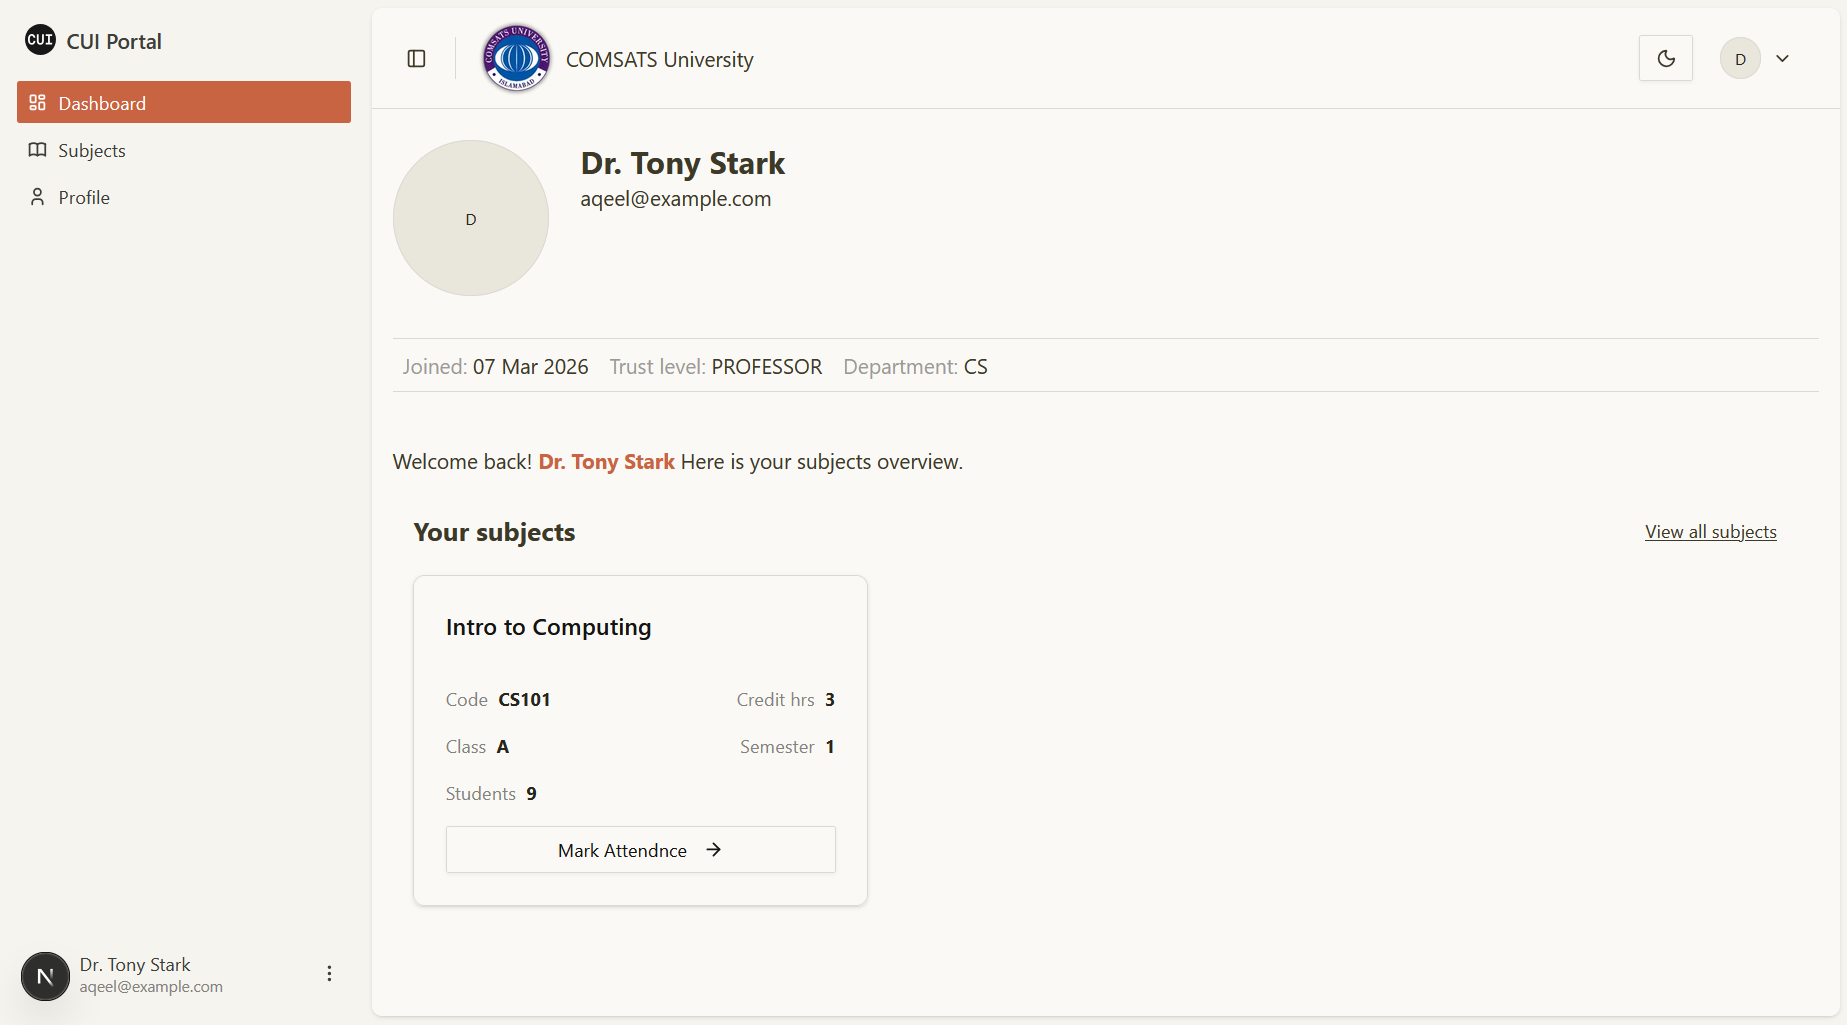
\includegraphics[width=\linewidth]{Figures/web/prf-das.png}
  \smallskip
  \textbf{Figure X:} Professor dashboard on desktop screen.
\end{center}
\begin{center}
  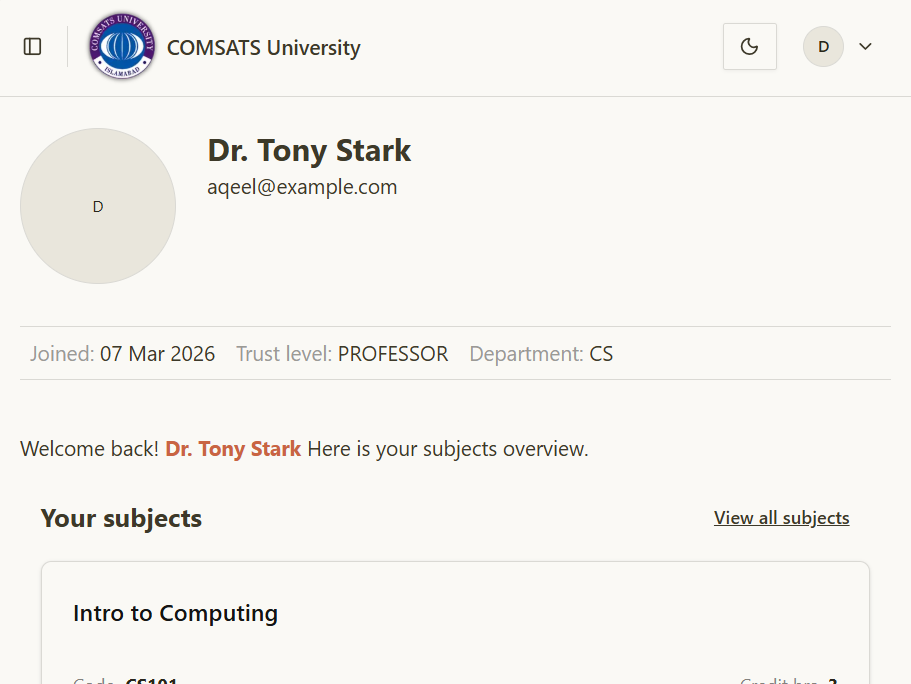
\includegraphics[width=\linewidth]{Figures/web/prf-das-mob.png}
  \smallskip
  \textbf{Figure X:} Professor dashboard on mobile screen.
\end{center}

    \item \textbf{Header:}
\begin{itemize}
    \item Large screens (desktop) show header links expanded.
    \item Smaller screens (mobile) show header collapsed by default which can be toggled using menu icon.
\end{itemize}
\end{itemize}

\textbf{Loading time optimization:}

\begin{itemize}
    \item \textbf{Strategic Suspense Boundaries \& Skeleton Loaders:} Implements the wrapper-renders-first pattern across all portal roles. The page shell and core UI elements paint immediately, while data-heavy tables are deferred using dedicated skeleton components (e.g., \texttt{AtRiskStudentsTableSkeleton}), ensuring faster initial layouts.
    \item \textbf{Parallel Independent Database Queries:} Utilizes \texttt{Promise.all()} to concurrently fetch lists and their total counts alongside required relations (e.g., in \texttt{get-complaints.ts}). This eliminates sequential waterfalls and reduces database round-trips, making data-heavy routes significantly faster.
    \item \textbf{Per-Request Deduplication:} Wraps global authorization checks (e.g., \texttt{requireSession}) in \texttt{React.cache()}. If multiple React Server Components on a single page request the user session natively, the database query executes exactly once.
    \item \textbf{Non-Blocking UI Transitions:} Heavily utilizes \texttt{useTransition} for parameter updates via \texttt{nuqs} and form submissions. The interface remains fully interactive instead of freezing while Next.js fetches fresh Server Component payloads for sorting, filtering, or pagination.
    \item \textbf{Asynchronous Sidebar Streaming:} Isolates non-critical peripheral data, such as sidebar announcements, within \texttt{Suspense} boundaries. This ensures that slow auxiliary fetches never block the main content's rendering pipeline.
\end{itemize}


\textbf{State management Strategy:}

\textbf{Responsiveness}
\begin{itemize}
    \item \textbf{Instant UI feedback:} \texttt{useState} and \texttt{useReducer} updates are synchronous and local, resulting in zero network delay for toggles, form changes, modals, and sorting UI.
    \item \textbf{URL-driven state:} Using \texttt{nuqs} keeps filters, pagination, and sorting in the URL, ensuring that page reloads or shareable links maintain the exact state without requiring additional fetches.
    \item \textbf{Snappy transitions:} Client-side transitions are highly responsive because the Next.js App Router combined with Server Components only re-renders the changed parts when parameters update.
    \item \textbf{Navigation consistency:} Drawer/sheet modals, tabs, and collapsible sections re-open correctly on back/forward navigation due to reliable URL synchronization.
\end{itemize}

\textbf{Performance}
\begin{itemize}
    \item \textbf{Minimal re-renders:} \texttt{useState} and \texttt{useReducer} localize updates, affecting only the owning component or its subtree.
    \item \textbf{Efficient parsing:} \texttt{nuqs} parsers run on the server once per request, removing any client-side parsing overhead during the initial payload load.
    \item \textbf{Lightweight hooks:} The \texttt{useQueryStates} hook is negligible in size ($\sim$3--5 KB gzipped), automatically memoized, and prevents unnecessary re-renders when unrelated parameters change.
    \item \textbf{No global store footprint:} Avoiding a global state store removes the unnecessary subscription overhead across unrelated components.
    \item \textbf{Data freshness:} Server Components fetch fresh data on parameter changes, naturally avoiding the stale client cache issues that are common in pure client-side state management architectures.
    \item \textbf{Near-zero bundle impact:} Combining \texttt{nuqs} with built-in React hooks keeps the client JavaScript bundle extremely small.
\end{itemize}


% -------------------------------------------------
% 5.6 Deployment
% -------------------------------------------------

\section{Deployment}

This section describes the deployment platforms and architectural services used in the project.

\begin{table}[h]
\centering
\renewcommand{\arraystretch}{1.5}
\caption{Deployment \& Infrastructure Details}
\begin{tabularx}{\textwidth}{|p{3.5cm}|p{3cm}|X|}
\hline
\textbf{Component} & \textbf{Platform} & \textbf{Details} \\
\hline
Frontend \& Backend (Next.js) & Vercel & Fully managed serverless deployment handling the React UI, Server Actions, API routes, and edge caching. \\
\hline
Database \& Storage & Neon Serverless Postgres & Managed serverless PostgreSQL database connected via Prisma ORM for auto-scaling and connection pooling. \\
\hline
Background Jobs \& Workflows & Inngest & Event-driven durable execution engine used to manage deferred operations (e.g., scheduled announcements). \\
\hline
Security \& Bot Protection & Arcjet dashboard & Integrated security layer for rate limiting, bot detection, and malicious request blocking directly within the Next.js middleware. \\
\hline
\end{tabularx}
\end{table}



%%%%%%%%%%%%%%%%%%%%%%%%%%%%%%%%%%%%%%%%%%%%%%%%%%%%%%
\section{Chapter Summary}
%%%%%%%%%%%%%%%%%%%%%%%%%%%%%%%%%%%%%%%%%%%%%%%%%%%%%%

This chapter presented the detailed implementation of the proposed system. 
The conceptual design and architectural models discussed in the previous chapter 
were translated into practical software components, including backend services, 
core functional modules, algorithmic engines, and user interface elements.

The development environment and configuration were described to ensure 
reproducibility of the implementation process. Each major module was implemented 
in a modular and loosely coupled manner to enhance maintainability and scalability. 
The core prediction algorithm was integrated into the system backend, enabling 
real-time processing of user input and generation of classification results.

External APIs and SDK integrations were discussed where applicable, 
highlighting authentication mechanisms and secure communication practices. 
The user interface implementation was explained screen-by-screen, including 
validation logic, navigation flow, and backend integration.

Finally, deployment strategies were presented, detailing hosting platforms, 
server configuration, and production setup. Overall, this chapter demonstrates 
the successful realization of the proposed system into a functional, 
deployable solution ready for testing and evaluation.
